

\setcounter{chapter}{2}

\chapter{商群与同态}

\section{定义和例子}

在本章中，我们引入群 \(G\) 的\textbf{商群}的概念，这是从群 \(G\) 得到“更小”群的另一种方式，并且正如我们对子群所做的那样，我们将利用商群来研究 \(G\) 的结构。群 \(G\) 的结构反映在 \(G\) 的商群和子群的结构中。例如，我们将看到，\(G\) 的\textbf{商}的子群格反映在 \(G\) 的格的“顶部”（在精确的意义上），而 \(G\) 的\textbf{子群}的格则自然地出现在“底部”。因此，通过结合这些信息，人们可以获得关于群 \(G\) 的信息，我们将指出一些分类定理是如何以这种方式产生的。

对 \(G\) 的商群的研究本质上等价于对 \(G\) 的同态的研究，即保持群结构的从群 \(G\) 到另一个群的映射。若 \(\varphi\) 是从 \(G\) 到群 \(H\) 的同态，回忆 \(\varphi\) 的\textbf{纤维}是 \(G\) 中投影到 \(H\) 的单个元素的元素集合，我们可以在图 1 中形象地表示，其中点 \(a\) 上方方框中的竖线表示 \(\varphi\) 在 \(a\) 上的纤维。


\begin{figure}[htbp]
    \centering
    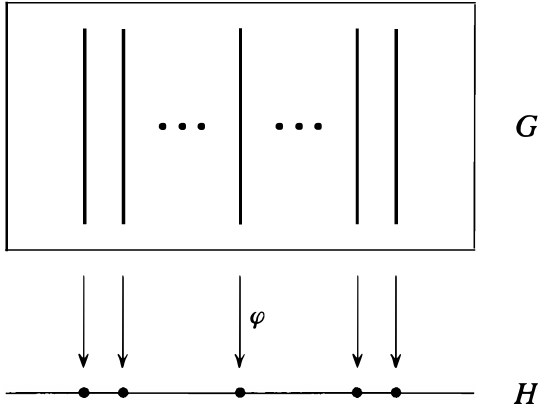
\includegraphics[width=0.5\textwidth]{images/fig3-1.png}
    \caption{}
    \label{fig3-1}
\end{figure}

\(H\) 中的群运算提供了一种将 \(\varphi\) 的像中的两个元素（即图 1 中水平线上的两个元素）相乘的方法。这提示我们对位于这两个点上方的纤维进行自然的乘法，从而将纤维的集合做成一个群：若 \(X_a\) 是 \(a\) 上方的纤维，\(X_b\) 是 \(b\) 上方的纤维，则 \(X_a\) 与 \(X_b\) 的乘积定义为乘积 \(ab\) 上方的纤维 \(X_{ab}\)，即 \(X_a X_b = X_{ab}\). 这个乘法是结合的，因为 \(H\) 中的乘法是结合的，单位元是 \(H\) 的单位元上方的纤维，而 \(a\) 上方的纤维的逆元是 \(a^{-1}\) 上方的纤维，这从定义容易验证。例如，结合律证明如下：\((X_a X_b)X_c = (X_{ab})X_c = X_{(ab)c}\) 且 \(X_a(X_b X_c) = X_a(X_{bc}) = X_{a(bc)}\). 由于在 \(H\) 中 \((ab)c = a(bc)\)，故 \((X_a X_b)X_c = X_a(X_b X_c)\). 粗略地说，群 \(G\) 被分成若干块（纤维），而这些块本身具有群的结构，称为 \(G\) 的一个\textbf{商群}（正式定义见下面例子之后）。

由于纤维的乘法是由 \(H\) 中的乘法定义的，根据构造，带有这个乘法的商群自然同构于 \(G\) 在同态 \(\varphi\) 下的像（纤维 \(X_a\) 与它在 \(H\) 中的像 \(a\) 等同）。

\begin{example}
设 \(G = \mathbb{Z}\)，令 \(H = Z_n = \langle x \rangle\) 为 \(n\) 阶循环群，并定义 \(\varphi : \mathbb{Z} \to Z_n\) 为 \(\varphi(a) = x^a\). 由于
\[
\varphi(a + b) = x^{a+b} = x^a x^b = \varphi(a)\varphi(b),
\]
可知 \(\varphi\) 是同态（注意 \(\mathbb{Z}\) 中的运算是加法，而 \(Z_n\) 中的运算是乘法）。还注意 \(\varphi\) 是满射。\(\varphi\) 在 \(x^a\) 上的纤维是
\[
\begin{aligned}
\varphi^{-1}(x^a) &= \{m \in \mathbb{Z} \mid x^m = x^a\} = \{m \in \mathbb{Z} \mid x^{m-a} = 1\} \\
&= \{m \in \mathbb{Z} \mid n \text{ 整除 } m - a\} \qquad \text{（由命题 2.3）} \\
&= \{m \in \mathbb{Z} \mid m \equiv a \pmod{n}\} = \bar{a},
\end{aligned}
\]
即 \(\varphi\) 的纤维恰好是模 \(n\) 的剩余类。此时图 1 变为：


\begin{figure}[htbp]
    \centering
    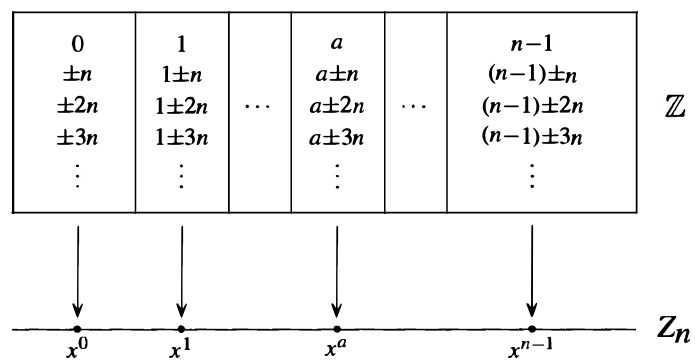
\includegraphics[width=0.75\textwidth]{images/fig3-2.png}
    \caption{}
    \label{fig3-2}
\end{figure}






\(Z_n\) 中的乘法就是 \(x^a x^b = x^{a+b}\). 相应的纤维是 \(\bar{a}, \bar{b}\) 和 \(\overline{a + b}\)，因此纤维上的群运算是 \(\bar{a} \cdot \bar{b} = \overline{a + b}\). 这恰好是加法下的群 \(\mathbb{Z}/n\mathbb{Z}\)，一个同构于 \(\varphi\) 的像（即整个 \(Z_n\)）的群。

这个群的单位元（\(Z_n\) 中单位元上方的纤维）由 \(\mathbb{Z}\) 中 \(n\) 的所有倍数组成，即 \(n\mathbb{Z}\)，它是 \(\mathbb{Z}\) 的一个\textbf{子群}，而其余纤维只是这个子群的平移 \(a + n\mathbb{Z}\). 群运算也可以直接通过在纤维中取\textbf{代表元}、在 \(\mathbb{Z}\) 中相加这些代表元并取包含该和的纤维来定义（这就是群 \(\mathbb{Z}/n\mathbb{Z}\) 原来的定义）。从计算的角度看，通过简单地相加代表元 \(a\) 和 \(b\) 来计算 \(\bar{a}\) 与 \(\bar{b}\) 的乘积，要比先计算这些纤维在 \(\varphi\) 下的像（即 \(x^a\) 和 \(x^b\)）、在 \(H\) 中将它们相乘（得到 \(x^{a+b}\)）然后取该乘积上方的纤维容易得多。

\end{example}


我们首先考虑同态及其纤维的一些基本性质。位于 \(H\) 的单位元上方的同态 \(\varphi : G \to H\) 的纤维被赋予一个名称：

\begin{definition}
若 \(\varphi\) 是同态 \(\varphi : G \to H\)，则 \(\varphi\) 的\textbf{核}是集合
\[
\{g \in G \mid \varphi(g) = 1\},
\]
并记作 \(\ker \varphi\)（这里 \(1\) 是 \(H\) 的单位元）。
\end{definition}

\begin{proposition}\label{pro:3.1}
设 \(G\) 和 \(H\) 是群，\(\varphi : G \to H\) 是同态。
\begin{enumerate}[label=(\arabic*)]
\item \(\varphi(1_G) = 1_H\)，其中 \(1_G\) 和 \(1_H\) 分别是 \(G\) 和 \(H\) 的单位元。
\item 对所有 \(g \in G\)，\(\varphi(g^{-1}) = \varphi(g)^{-1}\)。
\item 对所有 \(n \in \mathbb{Z}\)，\(\varphi(g^n) = \varphi(g)^n\)。
\item \(\ker \varphi\) 是 \(G\) 的子群。
%1_G属于kerφ
\item \(\operatorname{im}(\varphi)\)，即 \(G\) 在 \(\varphi\) 下的像，是 \(H\) 的子群。
\end{enumerate}
\end{proposition}

\begin{proof}
(1) 由于 \(\varphi(1_G) = \varphi(1_G 1_G) = \varphi(1_G)\varphi(1_G)\)，消去律表明 (1) 成立。

(2) \(\varphi(1_G) = \varphi(gg^{-1}) = \varphi(g)\varphi(g^{-1})\)，且由 (1)，\(\varphi(1_G) = 1_H\)，因此
\[
1_H = \varphi(g)\varphi(g^{-1}).
\]
两边左乘 \(\varphi(g)^{-1}\) 并化简得 (2)。

(3) 这是对 \(n \in \mathbb{Z}^+\) 的归纳法的简单练习。由 (2)，结论 (3) 对 \(n\) 的负值也成立。

(4) 由于 \(1_G \in \ker \varphi\)，\(\varphi\) 的核非空。设 \(x, y \in \ker \varphi\)，即 \(\varphi(x) = \varphi(y) = 1_H\)。则
\[
\varphi(xy^{-1}) = \varphi(x)\varphi(y^{-1}) = \varphi(x)\varphi(y)^{-1} = 1_H 1_H^{-1} = 1_H,
\]
即 \(xy^{-1} \in \ker \varphi\)。由子群判别法，\(\ker \varphi \leq G\)。

(5) 由于 \(\varphi(1_G) = 1_H\)，\(H\) 的单位元在 \(\varphi\) 的像中，所以 \(\operatorname{im}(\varphi)\) 非空。若 \(x\) 和 \(y\) 在 \(\operatorname{im}(\varphi)\) 中，设 \(x = \varphi(a)\)，\(y = \varphi(b)\)，则由 (2) 有 \(y^{-1} = \varphi(b^{-1})\)，因此
\[
xy^{-1} = \varphi(a)\varphi(b^{-1}) = \varphi(ab^{-1})
\]
（因 \(\varphi\) 是同态）。所以 \(xy^{-1}\) 也在 \(\varphi\) 的像中，故由子群判别法，\(\operatorname{im}(\varphi)\) 是 \(H\) 的子群。
\end{proof}

我们现在可以定义一些与商群相关的术语。

\begin{definition}
设 \(\varphi : G \to H\) 是同态，核为 \(K\). \textbf{商群}或\textbf{因子群} \(G/K\)（读作 \(G\) 模 \(K\) 或简称 \(G \bmod K\)）是以 \(\varphi\) 的纤维为元素的群，其群运算如上定义：即若 \(X\) 是 \(a\) 上方的纤维，\(Y\) 是 \(b\) 上方的纤维，则 \(X\) 与 \(Y\) 的乘积定义为乘积 \(ab\) 上方的纤维。
\end{definition}

这个记号强调了一个事实：核 \(K\) 是群 \(G/K\) 中的单个元素，且我们将在下面（命题 \ref{pro:3.2}）看到，如同上面的 \(\mathbb{Z}/n\mathbb{Z}\) 情形，\(G/K\) 的其他元素只是核 \(K\) 的“平移”。因此我们可以把 \(G/K\) 看作通过坍缩或“除以” \(K\)（更确切地说，通过模 \(K\) 的等价关系）得到的。这解释了为什么 \(G/K\) 被称为“商”群。

上面商群 \(G/K\) 的定义需要明确给出映射 \(\varphi\)，因为纤维的乘法是通过先用 \(\varphi\) 将纤维投影到 \(H\)，在 \(H\) 中相乘，然后确定该乘积上方的纤维来进行的。正如上面的 \(\mathbb{Z}/n\mathbb{Z}\) 情形，也可以直接用纤维中的代表元来定义纤维的乘法。这在计算上更简单，且映射 \(\varphi\) 不显式出现。我们首先说明同态的纤维可以像上面的例子那样用同态的核来表示（那里核是 \(n\mathbb{Z}\)，纤维是形如 \(a + n\mathbb{Z}\) 的平移）。

\begin{proposition}\label{pro:3.2}
设 \(\varphi : G \to H\) 是群同态，核为 \(K\). 设 \(X \in G/K\) 是 \(a\) 上方的纤维，即 \(X = \varphi^{-1}(a)\). 则
\begin{enumerate}[label=(\arabic*)]
\item 对任意 \(u \in X\)，\(X = \{uk \mid k \in K\}\).
\item 对任意 \(u \in X\)，\(X = \{ku \mid k \in K\}\).
\end{enumerate}
\end{proposition}

\begin{proof}
我们证明 (1)，把 (2) 的证明留作练习。设 \(u \in X\)，则由 \(X\) 的定义，\(\varphi(u) = a\). 令
\[
uK = \{uk \mid k \in K\}.
\]
首先证明 \(uK \subseteq X\). 对任意 \(k \in K\)，
\[
\begin{aligned}
\varphi(uk) &= \varphi(u)\varphi(k) && \text{（因 } \varphi \text{ 是同态）} \\
&= \varphi(u)1 && \text{（因 } k \in \ker \varphi\text{）} \\
&= a,
\end{aligned}
\]
即 \(uk \in X\). 这证明了 \(uK \subseteq X\). 为证反向包含，设 \(g \in X\)，令 \(k = u^{-1}g\). 则
\[
\begin{aligned}
\varphi(k) &= \varphi(u^{-1})\varphi(g) = \varphi(u)^{-1}\varphi(g) && \text{（由命题 \ref{pro:3.1}）} \\
&= a^{-1}a = 1.
\end{aligned}
\]
因此 \(k \in \ker \varphi\). 由于 \(k = u^{-1}g\)，故 \(g = uk \in uK\)，这证明了包含 \(X \subseteq uK\). 于是 (1) 得证。
\end{proof}

命题 \ref{pro:3.2} 中用于描述同态 \(\varphi\) 的纤维的集合，对 \(G\) 的任意子群 \(K\) 都有定义，不必是某个同态的核（我们很快将确定一个子群成为这样的核的充要条件），并给出一个名称：

\begin{definition}
对任意 \(N \leq G\) 和任意 \(g \in G\)，令
\[
gN = \{gn \mid n \in N\} \quad \text{和} \quad Ng = \{ng \mid n \in N\},
\]
分别称为 \(N\) 在 \(G\) 中的\textbf{左陪集}和\textbf{右陪集}。陪集中的任意元素称为该陪集的\textbf{代表元}。
\end{definition}

我们已经在命题 \ref{pro:3.2} 中看到，若 \(N\) 是某个同态的核，且 \(g_1\) 是陪集 \(gN\) 的任意代表元，则 \(g_1N = gN\)（且若 \(g_1 \in Ng\)，则 \(Ng_1 = Ng\)）。我们将在下面命题 \ref{pro:3.4} 中看到，这个事实对任意子群 \(N\) 都成立，这解释了“代表元”这一术语。

若 \(G\) 是加法群，我们将用 \(g + N\) 和 \(N + g\) 分别表示 \(N\) 在 \(G\) 中以 \(g\) 为代表的左陪集和右陪集。一般地，我们可以把 \(N\) 在 \(G\) 中的左陪集 \(gN\) 看作 \(N\) 被 \(g\) 左平移。（读者可能想复习第 1.7 节习题 18，它证明了 \(N\) 在 \(G\) 中的右陪集恰好是 \(N\) 通过左乘法作用在 \(G\) 上的轨道。）

用这个定义来说，命题 \ref{pro:3.2} 表明同态的纤维是核的左陪集（也是核的右陪集），即商群 \(G/K\) 的元素是左陪集 \(gK\)，\(g \in G\)。在 \(\mathbb{Z}/n\mathbb{Z}\) 的例子中，商群中的乘法也可以用陪集的代表元来定义。下面的结果表明对一般的 \(G/K\) 同样成立（只要我们已知 \(K\) 是某个同态的核），即 \(G/K\) 中两个左陪集 \(X\) 和 \(Y\) 的乘积可通过选取 \(X\) 的任意代表元 \(u\)、\(Y\) 的任意代表元 \(v\)，在 \(G\) 中将 \(u\) 和 \(v\) 相乘，然后取陪集 \((uv)K\) 来计算。

\begin{theorem}\label{thm:3.3}
设 \(G\) 是群，\(K\) 是从 \(G\) 到另一个群的某个同态的核。则以 \(K\) 在 \(G\) 中的左陪集为元素、运算由
\[
uK \cdot vK = (uv)K
\]
定义的集合构成一个群 \(G/K\). 特别地，这个运算是良定义的，即若 \(u_1\) 是 \(uK\) 中的任意元素、\(v_1\) 是 \(vK\) 中的任意元素，则 \(u_1 v_1 \in uvK\)，亦即 \(u_1 v_1 K = uvK\)，因此该乘法不依赖于陪集代表元的选取。把“左陪集”换成“右陪集”，结论同样成立。
\end{theorem}

\begin{proof}
设 \(X, Y \in G/K\)，令 \(Z = XY\) 为 \(G/K\) 中的乘积，于是由命题 \ref{pro:3.2}(1) 知 \(X, Y, Z\) 都是 \(K\) 的（左）陪集。由假设，\(K\) 是某个同态 \(\varphi : G \to H\) 的核，故 \(X = \varphi^{-1}(a)\)、\(Y = \varphi^{-1}(b)\)，其中 \(a, b \in H\). 由 \(G/K\) 中运算的定义，\(Z = \varphi^{-1}(ab)\). 设 \(u, v\) 分别为 \(X, Y\) 的任意代表元，于是 \(\varphi(u) = a\)、\(\varphi(v) = b\)，并且 \(X = uK\)、\(Y = vK\). 我们要证明 \(uv \in Z\). 由于
\[
uv \in Z \iff uv \in \varphi^{-1}(ab) \iff \varphi(uv) = ab \iff \varphi(u)\varphi(v) = ab,
\]
而最后一个等式确实成立，故 \(uv \in Z\)，从而 \(Z\) 是（左）陪集 \(uvK\).（下面的习题 2 反过来表明，每个 \(Z\) 都可以写成 \(uv\) 的形式，其中 \(u \in X\)、\(v \in Y\)。）这就证明了：对任意选取的代表元 \(u \in X\)、\(v \in Y\)，\(X\) 与 \(Y\) 的乘积都是陪集 \(uvK\)，从而完成了定理前一部分的证明。定理的最后一句立即成立，因为由命题 \ref{pro:3.2} 知对所有 \(u, v \in G\) 都有 \(uK = Ku\) 与 \(vK = Kv\).
\end{proof}

用图 1 的说法，通过代表元计算 \(G/K\) 中的乘法可以用下面的图 3 来表示。

\begin{figure}[htbp]
    \centering
    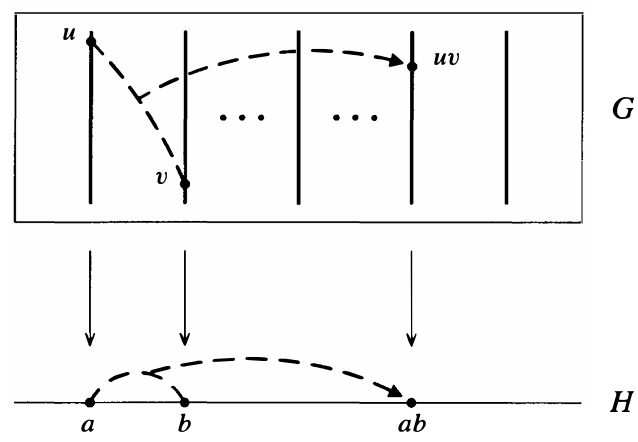
\includegraphics[width=0.5\textwidth]{images/fig3-3.png}
    \caption{}
    \label{fig3-3}
\end{figure}

我们要强调，乘法与所选取的代表元无关。也就是说，两个陪集 \(X\) 与 \(Y\) 的乘积（若群用加法记号书写则为和）是包含乘积 \(uv\) 的陪集 \(uvK\)，其中 \(u\) 与 \(v\) 分别是陪集 \(X\) 与 \(Y\) 的任意代表元。这种只考虑包含某个元素的陪集、即“模 \(K\) 约化”的过程，正是我们在 \(\mathbb{Z}/n\mathbb{Z}\) 中一直做的事情。表示包含代表元 \(u\) 的陪集 \(uK\) 的一个有用记号是 \(\bar{u}\). 采用这个记号（我们在预备知识中处理 \(\mathbb{Z}/n\mathbb{Z}\) 时已经引入过），商群 \(G/K\) 记作 \(\bar{G}\)，而元素 \(\bar{u}\) 与 \(\bar{v}\) 的乘积就是包含 \(uv\) 的陪集，即 \(\overline{uv}\). 这个记号也强化了如下事实：\(G/K\) 中的陪集 \(uK\) 正是 \(G/K\) 中的元素 \(\bar{u}\).

\begin{example}
（1）本章第一个例子中从 \(\mathbb{Z}\) 到 \(Z_n\) 的同态 \(\varphi\) 的纤维是核 \(n\mathbb{Z}\) 的左陪集（也是右陪集）\(a + n\mathbb{Z}\). 定理 \ref{thm:3.3} 证明这些陪集在代表元的加法下构成一个群，即 \(\mathbb{Z}/n\mathbb{Z}\)，这解释了该群的记号。这个群自然同构于它在 \(\varphi\) 下的像，于是我们重新得到了第 2 章的 \(\mathbb{Z}/n\mathbb{Z} \cong Z_n\).

（2）若 \(\varphi : G \to H\) 是同构，则 \(K = 1\)，\(\varphi\) 的纤维都是 \(G\) 的单点子集，于是 \(G/1 \cong G\).

（3）设 \(G\) 是任意群，\(H = 1\) 是 1 阶群，并定义 \(\varphi : G \to H\) 为对所有 \(g \in G\) 有 \(\varphi(g) = 1\). 立即看出 \(\varphi\) 是同态。这个映射称为\textbf{平凡同态}。注意此时 \(\ker \varphi = G\)，而 \(G/G\) 是只含一个元素 \(G\) 的群，即 \(G/G \cong Z_1 = \{1\}\).

（4）设 \(G = \mathbb{R}^2\)（运算为向量加法），\(H = \mathbb{R}\)（运算为加法），定义 \(\varphi : \mathbb{R}^2 \to \mathbb{R}\) 为 \(\varphi((x, y)) = x\). 于是 \(\varphi\) 是到 \(x\) 轴上的投影。我们证明 \(\varphi\) 是同态：
\[
\varphi((x_1, y_1) + (x_2, y_2)) = \varphi((x_1 + x_2, y_1 + y_2)) = x_1 + x_2 = \varphi((x_1, y_1)) + \varphi((x_2, y_2)).
\]
此时
\[
\ker \varphi = \{(x, y) \mid \varphi((x, y)) = 0\} = \{(x, y) \mid x = 0\} = y \text{ 轴}.
\]
注意 \(\ker \varphi\) 确实是 \(\mathbb{R}^2\) 的子群，且 \(\varphi\) 在 \(a \in \mathbb{R}\) 上方的纤维是把 \(y\) 轴平移 \(a\) 得到的直线 \(x = a\). 这也是核的一个左陪集（也是右陪集），以 \((a, 0)\)（或任何其他投影到 \(a\) 的代表点）为代表：
\[
(a, 0) + y \text{ 轴} = \overline{(a, 0)}.
\]
于是本例中的图 1 变为

\begin{figure}[htbp]
    \centering
    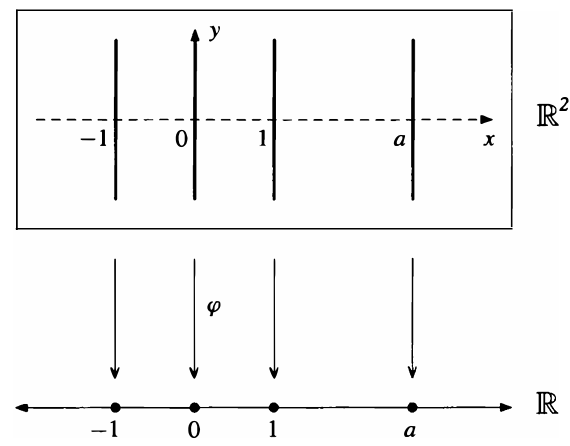
\includegraphics[width=0.5\textwidth]{images/fig3-4.png}
    \caption{}
    \label{fig3-4}
\end{figure}

群运算（此处用加法书写）既可以用映射 \(\varphi\) 来描述：直线 \((x = a)\) 与直线 \((x = b)\) 的和是直线 \((x = a + b)\)；也可以直接用陪集的代表元来描述：包含点 \((a, y_1)\) 的竖直线与包含点 \((b, y_2)\) 的竖直线的和是包含点 \((a + b, y_1 + y_2)\) 的竖直线。特别要注意，这些竖直线的代表元的选取并不重要（即 \(y\) 坐标无关紧要）。

（5）\(G = Q_8\)（四元数群，见第 2.5 节例 2），\(H = V_4\)（克莱因四元群）。定义 \(\varphi : Q_8 \to V_4\) 为
\[
\varphi(\pm 1) = 1, \quad \varphi(\pm i) = a, \quad \varphi(\pm j) = b, \quad \varphi(\pm k) = c.
\]
验证 \(\varphi\) 是同态留作练习——利用对称性可以最大限度地减少证明对所有 \(x, y \in Q_8\) 有 \(\varphi(xy) = \varphi(x)\varphi(y)\) 的工作量。显然 \(\varphi\) 是满射，且 \(\ker \varphi = \{\pm 1\}\). 可以把 \(\varphi\) 想成 \(Q_8\) 上的“绝对值”函数，于是 \(\varphi\) 的纤维是集合 \(E = \{\pm 1\}\)、\(A = \{\pm i\}\)、\(B = \{\pm j\}\)、\(C = \{\pm k\}\)，它们在 \(Q_8/\{\pm 1\}\) 中分别被坍缩为 \(1, a, b, c\)，而这些正是 \(\ker \varphi\) 的左陪集（也是右陪集）（例如 \(A = i \ker \varphi = \{i, -i\} = \ker \varphi \cdot i\)）。
\end{example}

由定理 \ref{thm:3.3}，如果我们已知群 \(G\) 的一个子群 \(K\) 是某个同态的核，就可以不借助该同态、直接用乘法 \(uK \cdot vK = uvK\) 来定义商群 \(G/K\). 这就引出一个问题：是否可以对 \(G\) 的任意子群 \(N\) 类似地定义商群 \(G/N\)？一般说来答案是否定的，因为该乘法一般不是良定义的（参见后面的命题 \ref{pro:3.5}）。事实上我们将看到，当且仅当 \(N\) 是某个同态的核时，才能在 \(N\) 的陪集上定义群结构（命题 \ref{pro:3.7}）。我们还将给出一个判别准则来判断子群 \(N\) 是否是这样一个核——这就是\textbf{正规子群}的概念，我们将在后续各节中考察非正规子群。

我们首先证明，\(G\) 的任意子群的陪集都划分 \(G\)（即它们的并是整个 \(G\)，且不同的陪集交为平凡）。

\begin{proposition}\label{pro:3.4}
设 \(N\) 是群 \(G\) 的任意子群。\(N\) 在 \(G\) 中的左陪集构成 \(G\) 的一个划分。此外，对所有 \(u, v \in G\)，\(uN = vN\) 当且仅当 \(v^{-1}u \in N\)；特别地，\(uN = vN\) 当且仅当 \(u\) 与 \(v\) 是同一陪集的代表元。
\end{proposition}

\begin{proof}
首先注意，由于 \(N\) 是 \(G\) 的子群，故 \(1 \in N\). 于是对所有 \(g \in G\) 有 \(g = g \cdot 1 \in gN\)，即
\[
G = \bigcup_{g \in G} gN.
\]
为证不同的左陪集交为空，设 \(uN \cap vN \neq \varnothing\)，我们证明 \(uN = vN\). 设 \(x \in uN \cap vN\)，写成
\[
x = un = vm, \quad \text{其中 } n, m \in N.
\]
在后一个等式中两边右乘 \(n^{-1}\)，得
\[
u = vm_1, \quad \text{其中 } m_1 = mn^{-1} \in N.
\]
现在对 \(uN\) 中的任意元素 \(ut\)（\(t \in N\)），
\[
ut = (vm_1)t = v(m_1 t) \in vN.
\]
这证明 \(uN \subseteq vN\). 交换 \(u\) 与 \(v\) 的角色，类似地得到 \(vN \subseteq uN\). 因此交集非空的两个陪集相同。

由命题的前一部分，\(uN = vN\) 当且仅当 \(u \in vN\)，当且仅当存在 \(n \in N\) 使 \(u = vn\)，当且仅当 \(v^{-1}u \in N\)，这正是所断言的。最后，\(v \in uN\) 等价于说 \(v\) 是 \(uN\) 的代表元，因此 \(uN = vN\) 当且仅当 \(u\) 与 \(v\) 是同一陪集（即陪集 \(uN = vN\)）的代表元。
\end{proof}

\begin{proposition}\label{pro:3.5}
设 \(G\) 是群，\(N\) 是 \(G\) 的子群。

\begin{enumerate}[label=(\arabic*)]
\item 由
\[
uN \cdot vN = (uv)N
\]
给出的 \(N\) 在 \(G\) 中的左陪集集合上的运算良定义，当且仅当对所有 \(g \in G\) 和所有 \(n \in N\) 都有 \(gng^{-1} \in N\).

\item 若上述运算良定义，则它使 \(N\) 在 \(G\) 中的左陪集集合成为一个群。特别地，该群的单位元是陪集 \(1N\)，\(gN\) 的逆元是陪集 \(g^{-1}N\)，即 \((gN)^{-1} = g^{-1}N\).
\end{enumerate}
\end{proposition}

\begin{proof}
（1）首先假设该运算良定义，即对所有 \(u, v \in G\)，若 \(u, u_1 \in uN\) 且 \(v, v_1 \in vN\)，则 \(uvN = u_1 v_1 N\).

设 \(g\) 是 \(G\) 的任意元素，\(n\) 是 \(N\) 的任意元素。令 \(u = 1\)、\(u_1 = n\)、\(v = v_1 = g^{-1}\)，应用上述假设推得
\[
1 \cdot g^{-1}N = ng^{-1}N, \quad \text{即 } g^{-1}N = ng^{-1}N.
\]
由于 \(1 \in N\)，故 \(ng^{-1} \cdot 1 \in ng^{-1}N\). 于是 \(ng^{-1} \in g^{-1}N\)，从而对某个 \(n_1 \in N\) 有 \(ng^{-1} = g^{-1}n_1\). 两边左乘 \(g\) 得 \(gng^{-1} = n_1 \in N\)，这正是所断言的。

反之，假设对所有 \(g \in G\) 和所有 \(n \in N\) 都有 \(gng^{-1} \in N\). 为证上述运算良定义，设 \(u, u_1 \in uN\) 且 \(v, v_1 \in vN\). 我们可以写成
\[
u_1 = un, \quad v_1 = vm, \quad \text{其中 } n, m \in N.
\]
我们必须证明 \(u_1 v_1 \in uvN\)：
\[
u_1 v_1 = (un)(vm) = u(vv^{-1})nvm = (uv)(v^{-1}nv)m = (uv)(n_1 m),
\]
其中 \(n_1 = v^{-1}nv = (v^{-1})n(v^{-1})^{-1}\) 由假设是 \(N\) 的元素。由于 \(N\) 对乘法封闭，故 \(n_1 m \in N\). 于是
\[
u_1 v_1 = (uv)n_2, \quad \text{其中 } n_2 \in N.
\]
因此左陪集 \(uvN\) 与 \(u_1 v_1 N\) 含有公共元素 \(u_1 v_1\). 由前一个命题，它们相等。这证明该运算良定义。

（2）若陪集上的运算良定义，则群公理容易验证，它们由在 \(G\) 中的有效性诱导而来。例如，结合律成立，因为对所有 \(u, v, w \in G\)，
\[
(uN)(vN \cdot wN) = uN(vwN) = u(vw)N = (uv)wN = (uN \cdot vN)(wN),
\]
这是因为在 \(G\) 中 \(u(vw) = (uv)w\). \(G/N\) 中的单位元是陪集 \(1N\)，而 \(gN\) 的逆元是 \(g^{-1}N\)，这从乘法的定义立即得到。
\end{proof}

如前所述，满足命题 \ref{pro:3.5} 中条件、使得商 \(G/N\) 上有自然群结构的子群 \(N\) 被赋予一个名称：

\begin{definition}
元素 \(gng^{-1}\) 称为 \(n \in N\) 被 \(g\) 的\textbf{共轭}。集合 \(gNg^{-1} = \{gng^{-1} \mid n \in N\}\) 称为 \(N\) 被 \(g\) 的共轭。若 \(gNg^{-1} = N\)，则称元素 \(g\) \textbf{正规化} \(N\). 群 \(G\) 的子群 \(N\) 称为\textbf{正规的}，若 \(G\) 的每个元素都正规化 \(N\)，即对所有 \(g \in G\) 有 \(gNg^{-1} = N\). 若 \(N\) 是 \(G\) 的正规子群，我们记作 \(N \trianglelefteq G\).
\end{definition}

注意，当 \(N\) 是正规子群时，\(G\) 的结构反映在商 \(G/N\) 的结构中（例如，\(G/N\) 中乘法的结合律由 \(G\) 中的结合律诱导，\(G/N\) 中的逆元由 \(G\) 中的逆元诱导）。当我们在后面的 3.3 节考虑同构定理时，将进一步看到 \(G\) 与其商 \(G/N\) 的关系。

我们把上面的结果总结为定理 \ref{thm:3.6}.

\begin{theorem}\label{thm:3.6}
设 \(N\) 是群 \(G\) 的子群。下列命题等价：

\begin{enumerate}[label=(\arabic*)]
\item \(N \trianglelefteq G\)；

\item \(N_G(N) = G\)（回忆 \(N_G(N)\) 是 \(N\) 在 \(G\) 中的正规化子）；

\item 对所有 \(g \in G\) 有 \(gN = Ng\)；

\item 命题 \ref{pro:3.5} 中描述的 \(N\) 在 \(G\) 中的左陪集上的运算使这些左陪集构成一个群；

\item 对所有 \(g \in G\) 有 \(gNg^{-1} \subseteq N\).
\end{enumerate}
\end{theorem}

\begin{proof}
困难的等价性我们已经完成了，其余留作练习。
\end{proof}

作为一个实际问题，人们会设法尽量减少判断给定子群 \(N\) 在群 \(G\) 中是否正规所需的计算。特别地，人们尽量不计算所有共轭 \(gng^{-1}\)（\(n \in N\)，\(g \in G\)）。例如，\(N\) 自身的元素都正规化 \(N\)，因为 \(N\) 是子群。此外，如果已知 \(N\) 的一组生成元，则只需验证这些生成元的所有共轭都落在 \(N\) 中，就可证明 \(N\) 是正规子群（这是因为乘积的共轭是共轭的乘积，而逆元的共轭是共轭的逆元）——这就是后面的习题 26. 类似地，如果也知道 \(G\) 的生成元，则只需验证这些 \(G\) 的生成元都正规化 \(N\). 特别地，如果 \(N\) 和 \(G\) 的生成元都已知，这就把计算减少到少量需要验证的共轭。若 \(N\) 是有限群，则只需验证 \(N\) 的一组生成元被 \(G\) 的一组生成元共轭后仍属于 \(N\)（习题 29）。最后，常常可以直接证明 \(N_G(N) = G\) 而不必做过多计算（下一节有一些例子），这样也就证明了 \(N\) 是 \(G\) 的正规子群，而无需机械地计算所有可能的共轭 \(gng^{-1}\).

现在我们证明，正规子群恰好就是前面考虑的同态的核。

\begin{proposition}\label{pro:3.7}
群 \(G\) 的子群 \(N\) 正规，当且仅当它是某个同态的核。
\end{proposition}

\begin{proof}
若 \(N\) 是同态 \(\varphi\) 的核，则由命题 \ref{pro:3.2} 知 \(N\) 的左陪集与右陪集相同（二者都是映射 \(\varphi\) 的纤维）。于是由定理 \ref{thm:3.6}(3) 知 \(N\) 是正规子群。（对正规性的定义另有一个直接的证明，见习题。）

反之，若 \(N \trianglelefteq G\)，令 \(H = G/N\)，并由
\[
\pi(g) = gN, \quad \text{对所有 } g \in G
\]
定义 \(\pi : G \to G/N\). 由 \(G/N\) 中运算的定义，
\[
\pi(g_1 g_2) = (g_1 g_2)N = g_1 N \cdot g_2 N = \pi(g_1)\pi(g_2).
\]
这证明 \(\pi\) 是同态。此时
\[
\ker \pi = \{g \in G \mid \pi(g) = 1N\} = \{g \in G \mid gN = 1N\} = \{g \in G \mid g \in N\} = N.
\]
因此 \(N\) 是同态 \(\pi\) 的核。
\end{proof}

上面构造的、把正规子群 \(N\) 表示为某个同态的核的同态 \(\pi\) 被赋予一个名称：

\begin{definition}
设 \(N \trianglelefteq G\). 由 \(\pi(g) = gN\) 定义的（映到）同态 \(\pi : G \to G/N\) 称为 \(G\) 到 \(G/N\) 上的\textbf{自然投影}（同态）。若 \(\overline{H} \leq G/N\) 是 \(G/N\) 的子群，则它在 \(G\) 中的\textbf{完全原像}是 \(\overline{H}\) 在自然投影同态下的原像。
\end{definition}

\(G/N\) 的子群的完全原像是 \(G\) 的子群（参见习题 1），它包含子群 \(N\)，因为这些正是映射到单位元的元素。我们将在 3.3 节的同构定理中看到，包含 \(N\) 的 \(G\) 的子群与商 \(G/N\) 的子群之间存在自然的对应关系。

现在我们有一条“内部的”判别准则，它精确地刻画了给定群 \(G\) 的子群 \(N\) 何时是某个同态的核，即
\[
N_G(N) = G.
\]
因此我们可以把 \(G\) 的子群 \(N\) 的正规化子看作衡量 \(N\) “离正规子群有多近”的尺度（这解释了该子群的名称）。请记住，正规性是一个嵌入性质，即它依赖于 \(N\) 与 \(G\) 的关系，而不依赖于 \(N\) 自身的内部结构（同一个群 \(N\) 可以是 \(G\) 的正规子群，但在包含 \(G\) 的更大群中不正规）。

我们是从 \(G\) 到 \(H\) 的同态 \(\varphi\) 的存在性开始讨论商群的，并证明了该同态的核是 \(G\) 的正规子群 \(N\)，而商 \(G/N\)（最初用纤维定义）自然同构于 \(G\) 在 \(\varphi\) 下的像\footnote{“自然”一词在范畴论中有精确的数学意义；就我们的目的而言，用这个词只是表明该同态的定义是一种“无坐标”的投影，即只用元素本身来描述，而不使用 \(G\) 或 \(N\) 的生成元（参见附录 II）。}。反之，若 \(N \trianglelefteq G\)，我们可以找到一个群 \(H\)（即 \(G/N\)）和一个同态 \(\pi : G \to H\)，使得 \(\ker \pi = N\)（即自然投影）。因此，对 \(G\) 的同态像（即 \(G\) 到其他群的同态的像）的研究等价于对 \(G\) 的商群的研究，我们将用同态来产生正规子群，反之亦然。

我们通过同态来发展商群的理论，而不是简单地定义正规子群及其商群的概念，是为了强调商群的元素是原群 \(G\) 的子集（核 \(N\) 的纤维或陪集）。图 1 的直观图示也强调 \(N\)（及其陪集）被投影（或坍缩）为商 \(G/N\) 中的单个元素。商群 \(G/N\) 中的计算是通过从所涉及的各个陪集中取代表元来完成的。

下面给出正规子群及其商的一些例子。

\begin{example}
设 \(G\) 是群。

（1）子群 \(1\) 和 \(G\) 总是 \(G\) 的正规子群；\(G/1 \cong G\)，\(G/G \cong 1\).

（2）若 \(G\) 是阿贝尔群，则 \(G\) 的任意子群 \(N\) 都正规，因为对所有 \(g \in G\) 和所有 \(n \in N\)，
\[
gng^{-1} = gg^{-1}n = n \in N.
\]
注意这里重要的是 \(G\) 阿贝尔，而不仅仅是 \(N\) 阿贝尔。当取 \(G\) 的不同子群 \(N\) 时，\(G/N\) 的结构可能不同。例如，若 \(G = \mathbb{Z}\)，则 \(G\) 的每个子群 \(N\) 都是循环的：
\[
N = \langle n \rangle = \langle -n \rangle = n\mathbb{Z}, \quad \text{对某个 } n \in \mathbb{Z},
\]
而 \(G/N = \mathbb{Z}/n\mathbb{Z}\) 是以 \(1 + n\mathbb{Z}\) 为生成元的循环群（注意 \(1\) 是 \(G\) 的生成元）。

现在设 \(G = Z_k\) 是 \(k\) 阶循环群。设 \(x\) 是 \(G\) 的生成元，\(N \leq G\). 由命题 2.6，\(N = \langle x^d \rangle\)，其中 \(d\) 是落在 \(N\) 中的 \(x\) 的最小幂。此时
\[
G/N = \{gN \mid g \in G\} = \{x^a N \mid a \in \mathbb{Z}\},
\]
且由于 \(x^a N = (xN)^a\)（见下面习题 4），可知
\[
G/N = \langle xN \rangle,
\]
即 \(G/N\) 是循环群，以 \(xN\) 为生成元。

由下面习题 5，\(xN\) 在 \(G/N\) 中的阶等于 \(d\). 由命题 2.5，\(d = |G : N|\). 总结如下：循环群的商群是循环群，且 \(G\) 的生成元 \(g\) 在商群中的像 \(\bar{g}\) 是商群的生成元。若此外 \(G\) 是有限循环群且 \(N \trianglelefteq G\)，则 \(|G/N| = |G : N|\) 给出了商群阶的公式。

（3）若 \(N \leq Z(G)\)，则 \(N \trianglelefteq G\)，因为对所有 \(g \in G\) 和所有 \(n \in N\) 有 \(gng^{-1} = n \in N\)，这是前一个例子的推广（其中中心 \(Z(G)\) 就是整个 \(G\)）。因此特别地，\(Z(G) \trianglelefteq G\). 前面已经看到 \(Q_8\) 的子群 \(\{-1\}\) 是某个同态的核，但由于 \(\{-1\} = Z(Q_8)\)，我们现在又用另一种方式得到了该子群的正规性。我们已经看到 \(Q_8/\{-1\} \cong V_4\). 下一段中关于 \(D_8\) 的讨论同样适用于 \(Q_8\)，从而可以独立地确定该商群的同构类型。

设 \(G = D_8\)，令 \(Z = \langle r^2 \rangle = Z(D_8)\). 由于 \(Z = \{1, r^2\}\)，每个陪集 \(gZ\) 都由二元素集合 \(\{g, gr^2\}\) 组成。由于这些陪集把 \(D_8\) 的 8 个元素分成四对，\(Z\) 在 \(D_8\) 中必有 4 个（互不相交的）左陪集：
\[
\bar{1} = 1Z, \quad \bar{r} = rZ, \quad \bar{s} = sZ, \quad \overline{rs} = rsZ.
\]
现在由 4 阶群的分类（第 2.5 节习题 10）知 \(D_8/Z(D_8) \cong Z_4\) 或 \(V_4\). 为确定究竟是哪一个（即确定该商群的同构类型），只需注意
\[
\bar{r}^2 = r^2 Z = 1Z = \bar{1}, \quad \bar{s}^2 = s^2 Z = 1Z = \bar{1}, \quad \overline{rs}^2 = (rs)^2 Z = 1Z = \bar{1},
\]
所以 \(D_8/Z\) 中每个非单位元都是 2 阶的。特别地，商群中没有 4 阶元，因此 \(D_8/Z\) 不是循环群，从而 \(D_8/Z(D_8) \cong V_4\).
\end{example}

\subsection*{习题}
设 \(G\) 和 \(H\) 是群。

\begin{enumerate}
\item 设 \(\varphi : G \to H\) 是同态，\(E\) 是 \(H\) 的子群。证明 \(\varphi^{-1}(E) \leq G\)（即子群在同态下的原像或拉回是子群）。若 \(E \trianglelefteq H\)，证明 \(\varphi^{-1}(E) \trianglelefteq G\). 由此推出 \(\ker \varphi \trianglelefteq G\).

\item 设 \(\varphi : G \to H\) 是核为 \(K\) 的群同态，\(a, b \in \varphi(G)\). 设 \(X \in G/K\) 是 \(a\) 上方的纤维，\(Y\) 是 \(b\) 上方的纤维，即 \(X = \varphi^{-1}(a)\)、\(Y = \varphi^{-1}(b)\). 固定 \(X\) 中的一个元素 \(u\)（故 \(\varphi(u) = a\)）。证明：若商群 \(G/K\) 中 \(XY = Z\)，且 \(w\) 是 \(Z\) 的任意元素，则存在 \(v \in Y\) 使得 \(uv = w\).〔提示：证明 \(u^{-1}w \in Y\).〕

\item 设 \(A\) 是阿贝尔群，\(B\) 是 \(A\) 的子群。证明 \(A/B\) 是阿贝尔群。给出一个含真正规子群 \(N\) 的非阿贝尔群 \(G\) 的例子，使得 \(G/N\) 是阿贝尔群。

\item 证明在商群 \(G/N\) 中，对所有 \(a \in \mathbb{Z}\) 有 \((gN)^a = g^a N\).

\item 利用前一习题证明：\(G/N\) 中元素 \(gN\) 的阶是使 \(g^n \in N\) 的最小正整数 \(n\)（若这样的正整数不存在，则 \(gN\) 是无限阶的）。给出一个例子说明 \(gN\) 在 \(G/N\) 中的阶可能严格小于 \(g\) 在 \(G\) 中的阶。

\item 定义 \(\varphi : \mathbb{R}^\times \to \{\pm 1\}\) 为 \(\varphi(x)\) 等于 \(x\) 除以 \(x\) 的绝对值。描述 \(\varphi\) 的纤维，并证明 \(\varphi\) 是同态。

\item 定义 \(\pi : \mathbb{R}^2 \to \mathbb{R}\) 为 \(\pi((x, y)) = x + y\). 证明 \(\pi\) 是满同态，并几何地描述 \(\pi\) 的核与纤维。

\item 设 \(\varphi : \mathbb{R}^\times \to \mathbb{R}^\times\) 是把 \(x\) 映到 \(x\) 的绝对值的映射。证明 \(\varphi\) 是同态，并求出 \(\varphi\) 的像。描述 \(\varphi\) 的核与纤维。

\item 定义 \(\varphi : \mathbb{C}^\times \to \mathbb{R}^\times\) 为 \(\varphi(a + bi) = a^2 + b^2\). 证明 \(\varphi\) 是同态，并求出 \(\varphi\) 的像。几何地描述 \(\varphi\) 的核与纤维（作为平面的子集）。

\item 定义 \(\varphi : \mathbb{Z}/8\mathbb{Z} \to \mathbb{Z}/4\mathbb{Z}\) 为 \(\varphi(\bar{a}) = \bar{a}\). 证明这是一个良定义的满同态，并具体描述它的纤维与核（证明 \(\varphi\) 良定义要用到 \(\bar{a}\) 在 \(\varphi\) 的定义域与值域中含义不同这一事实）。

\item 设 \(F\) 是域，令
\[
G = \left\{ \begin{pmatrix} a & b \\ 0 & c \end{pmatrix} \ \middle|\ a, b, c \in F,\ ac \neq 0 \right\} \leq GL_2(F).
\]
（a）证明映射 \(\varphi : \begin{pmatrix} a & b \\ 0 & c \end{pmatrix} \mapsto a\) 是 \(G\) 到 \(F^\times\) 上的满同态（回忆 \(F^\times\) 是 \(F\) 中非零元素构成的乘法群）。描述 \(\varphi\) 的纤维与核。

（b）证明映射 \(\psi : \begin{pmatrix} a & b \\ 0 & c \end{pmatrix} \mapsto (a, c)\) 是 \(G\) 到 \(F^\times \times F^\times\) 上的满同态。描述 \(\psi\) 的纤维与核。

（c）设 \(H = \left\{ \begin{pmatrix} 1 & b \\ 0 & 1 \end{pmatrix} \ \middle|\ b \in F \right\}\). 证明 \(H\) 同构于加法群 \(F\).

\item 设 \(G\) 是实数的加法群，\(H\) 是模为 1 的复数的乘法群（复平面上的单位圆 \(S^1\)），并设 \(\varphi : G \to H\) 是同态 \(\varphi : r \mapsto e^{2\pi i r}\). 画出实直线上落在 \(\varphi\) 的核中的点。类似地描述 \(\varphi\) 在 \(H\) 的点 \(-1\)、\(i\) 和 \(e^{4\pi i/3}\) 上方的纤维中的元素。（正文中这个同态 \(\varphi\) 的图 1 通常用下面的图表示。）

\begin{figure}[htbp]
    \centering
    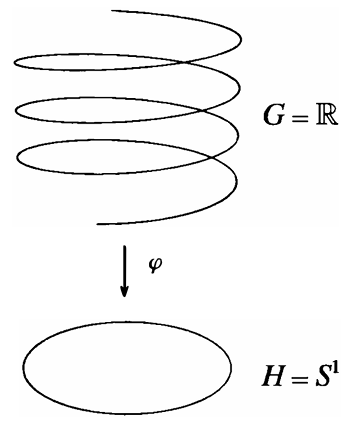
\includegraphics[width=0.5\textwidth]{images/fig3-5.png}
    \caption{}
    \label{fig3-5}
\end{figure}

\item 把前一习题中的映射 \(\varphi\) 换为 \(\varphi : r \mapsto e^{4\pi i r}\)，重复前一习题。

\item 考虑加法商群 \(\mathbb{Q}/\mathbb{Z}\).

（a）证明 \(\mathbb{Z}\) 在 \(\mathbb{Q}\) 中的每个陪集恰好含有一个满足 \(0 \leq q < 1\) 的代表元 \(q \in \mathbb{Q}\).

（b）证明 \(\mathbb{Q}/\mathbb{Z}\) 的每个元素都是有限阶的，但存在阶数任意大的元素。

（c）证明 \(\mathbb{Q}/\mathbb{Z}\) 是 \(\mathbb{R}/\mathbb{Z}\) 的挠子群（参见第 2.1 节习题 6）。

（d）证明 \(\mathbb{Q}/\mathbb{Z}\) 同构于 \(\mathbb{C}^\times\) 中的单位根乘法群。

\item 证明可除阿贝尔群对任意真子群的商仍是可除的。由此推出 \(\mathbb{Q}/\mathbb{Z}\) 可除（参见第 2.4 节习题 19）。

\item 设 \(G\) 是群，\(N\) 是 \(G\) 的正规子群，令 \(\bar{G} = G/N\). 证明：若 \(G = \langle x, y \rangle\)，则 \(\bar{G} = \langle \bar{x}, \bar{y} \rangle\). 更一般地证明：若对 \(G\) 的某个子集 \(S\) 有 \(G = \langle S \rangle\)，则 \(\bar{G} = \langle \bar{S} \rangle\).

\item 设 \(G\) 是 16 阶二面体群（其子群格见 2.5 节）：
\[
G = \langle r, s \mid r^8 = s^2 = 1,\ rs = sr^{-1} \rangle,
\]
并设 \(\bar{G} = G/\langle r^4 \rangle\) 是 \(G\) 对由 \(r^4\) 生成的子群的商（该子群是 \(G\) 的中心，因而正规）。

（a）证明 \(\bar{G}\) 的阶为 8.

（b）把 \(\bar{G}\) 的每个元素写成 \(s^a r^b\) 的形式（\(a, b\) 为整数）。

（c）求出（b）中所列 \(\bar{G}\) 每个元素的阶。

（d）把 \(\bar{G}\) 的下列每个元素写成 \(s^a r^b\) 的形式（\(a, b\) 如（b））：\(\overline{rs}\)、\(\overline{sr^{-2}s}\)、\(\overline{s^{-1}r^{-1}sr}\).

（e）证明 \(\bar{H} = \langle \bar{s}, \overline{r^2} \rangle\) 是 \(\bar{G}\) 的正规子群，且 \(\bar{H}\) 同构于克莱因四元群。描述 \(\bar{H}\) 在 \(G\) 中的完全原像的同构类型。

（f）求 \(\bar{G}\) 的中心，并描述 \(\bar{G}/Z(\bar{G})\) 的同构类型。

\item 设 \(G\) 是 16 阶拟二面体群（其子群格已在第 2.5 节习题 11 中算出）：
\[
G = \langle a, \tau \mid a^8 = \tau^2 = 1,\ a\tau = \tau a^3 \rangle,
\]
并设 \(\bar{G} = G/\langle a^4 \rangle\) 是 \(G\) 对由 \(a^4\) 生成的子群的商（该子群是 \(G\) 的中心，因而正规）。

（a）证明 \(\bar{G}\) 的阶为 8.

（b）把 \(\bar{G}\) 的每个元素写成 \(\tau^a a^b\) 的形式（\(a, b\) 为整数）。

（c）求出（b）中所列 \(\bar{G}\) 每个元素的阶。

（d）把 \(\bar{G}\) 的下列每个元素写成 \(\tau^a a^b\) 的形式（\(a, b\) 如（b））：\(\overline{a\tau}\)、\(\overline{\tau a^{-2}\tau}\)、\(\overline{\tau^{-1}a^{-1}\tau a}\).

（e）证明 \(\bar{G} \cong D_8\).

\item 设 \(G\) 是 16 阶模群（其子群格已在第 2.5 节习题 14 中算出）：
\[
G = \langle u, v \mid u^2 = v^8 = 1,\ vu = uv^5 \rangle,
\]
并设 \(\bar{G} = G/\langle v^4 \rangle\) 是 \(G\) 对由 \(v^4\) 生成的子群的商（该子群包含在 \(G\) 的中心中，因而正规）。

（a）证明 \(\bar{G}\) 的阶为 8.

（b）把 \(\bar{G}\) 的每个元素写成 \(u^a v^b\) 的形式（\(a, b\) 为整数）。

（c）求出（b）中所列 \(\bar{G}\) 每个元素的阶。

（d）把 \(\bar{G}\) 的下列每个元素写成 \(u^a v^b\) 的形式（\(a, b\) 如（b））：\(\overline{vu}\)、\(\overline{uv^{-2}u}\)、\(\overline{u^{-1}v^{-1}uv}\).

（e）证明 \(\bar{G}\) 是阿贝尔群，且同构于 \(Z_2 \times Z_4\).

\item 设 \(G = \mathbb{Z}/24\mathbb{Z}\)，令 \(\bar{G} = G/\langle \overline{12} \rangle\)，其中对每个整数 \(a\) 我们把 \(\bar{a}\) 简记为 \(a\).

（a）证明 \(\bar{G} = \{\bar{0}, \bar{1}, \ldots, \overline{11}\}\).

（b）求出 \(\bar{G}\) 中每个元素的阶。

（c）证明 \(\bar{G} \cong \mathbb{Z}/12\mathbb{Z}\).（于是 \((\mathbb{Z}/24\mathbb{Z})/(12\mathbb{Z}/24\mathbb{Z}) \cong \mathbb{Z}/12\mathbb{Z}\)，就像把 24 和 12 相除、约去 \(24/12\) 一样。）

\item 设 \(G = Z_4 \times Z_4\) 由如下生成元与关系给出：
\[
G = \langle x, y \mid x^4 = y^4 = 1,\ xy = yx \rangle.
\]
令 \(\bar{G} = G/\langle x^2 y^2 \rangle\)（注意阿贝尔群 \(G\) 的每个子群都正规）。

（a）证明 \(\bar{G}\) 的阶为 8.

（b）把 \(\bar{G}\) 的每个元素写成 \(x^a y^b\) 的形式（\(a, b\) 为整数）。

（c）求出（b）中所列 \(\bar{G}\) 每个元素的阶。

（d）证明 \(\bar{G} \cong Z_4 \times Z_2\).

\item （a）证明：若 \(H\) 和 \(K\) 是群 \(G\) 的正规子群，则它们的交 \(H \cap K\) 也是 \(G\) 的正规子群。

（b）证明：群的正规子群的任意非空族的交是正规子群（不要假设该族可数）。

\item 证明群的正规子群的任意非空族的并（参见第 2.5 节）是正规子群。

\item 证明：若 \(N \trianglelefteq G\)，\(H\) 是 \(G\) 的任意子群，则 \(N \cap H \trianglelefteq H\).

\item （a）证明 \(G\) 的子群 \(N\) 正规，当且仅当对所有 \(g \in G\) 有 \(gNg^{-1} \subseteq N\).

（b）设 \(G = GL_2(\mathbb{Q})\)，\(N\) 是对角线上为 1、元素为整数的上三角矩阵构成的子群，\(g\) 是以 2, 1 为对角元的对角矩阵。证明 \(gNg^{-1} \subseteq N\)，但 \(g\) 不正规化 \(N\).

\item 设 \(a, b \in G\).

（a）证明 \(a\) 与 \(b\) 的乘积的共轭等于 \(a\) 的共轭与 \(b\) 的共轭的乘积。证明 \(a\) 的阶与 \(a\) 的任意共轭的阶相同。

（b）证明 \(a^{-1}\) 的共轭是 \(a\) 的共轭的逆元。

（c）设对 \(G\) 的某个子集 \(S\) 有 \(N = \langle S \rangle\). 证明：若对所有 \(g \in G\) 有 \(gSg^{-1} \subseteq N\)，则 \(N \trianglelefteq G\).

（d）由此推出：若 \(N\) 是循环群 \(\langle x \rangle\)，则 \(N\) 在 \(G\) 中正规，当且仅当对每个 \(g \in G\) 存在 \(k \in \mathbb{Z}\) 使 \(gxg^{-1} = x^k\).

（e）设 \(n\) 是正整数。证明 \(G\) 的由所有 \(n\) 阶元素生成的子群 \(N\) 是 \(G\) 的正规子群。

\item 设 \(N\) 是群 \(G\) 的有限子群。证明 \(gNg^{-1} \subseteq N\) 当且仅当 \(gNg^{-1} = N\). 由此推出 \(N_G(N) = \{g \in G \mid gNg^{-1} \subseteq N\}\).

\item 设 \(N\) 是群 \(G\) 的有限子群，并假设对 \(G\) 的某个子集 \(S\) 有 \(N = \langle S \rangle\). 证明元素 \(g \in G\) 正规化 \(N\)，当且仅当 \(gSg^{-1} \subseteq N\).

\item 设 \(N\) 是 \(G\) 的有限子群，并假设存在 \(G\) 的子集 \(S, T\) 使得 \(G = \langle T \rangle\)、\(N = \langle S \rangle\). 证明 \(N\) 在 \(G\) 中正规，当且仅当对所有 \(t \in T\) 有 \(tSt^{-1} \subseteq N\).

\item 设 \(N \trianglelefteq G\)，\(g \in G\). 证明 \(gN = Ng\) 当且仅当 \(g \in N_G(N)\).

\item 证明：若 \(H \leq G\)，\(N\) 是 \(H\) 的正规子群，则 \(H \leq N_G(N)\). 由此推出 \(N_G(N)\) 是 \(G\) 中使 \(N\) 正规的最大子群（即所有使 \(N \trianglelefteq H\) 的子群 \(H\) 的并）。

\item 证明 \(Q_8\) 的每个子群都正规。对每个子群求出其对应商群的同构类型。〔可使用 2.5 节中 \(Q_8\) 的子群格。〕

\item 求出 \(D_8\) 的所有正规子群，并对其中每个求出对应商群的同构类型。〔可使用 2.5 节中 \(D_8\) 的子群格。〕

\item 设 \(D_{2n} = \langle r, s \mid r^n = s^2 = 1,\ rs = sr^{-1} \rangle\) 是 \(2n\) 阶二面体群的通常表示，\(k\) 是整除 \(n\) 的正整数。

（a）证明 \(\langle r^k \rangle\) 是 \(D_{2n}\) 的正规子群。

（b）证明 \(D_{2n}/\langle r^k \rangle \cong D_{2k}\).

\item 证明 \(SL_n(F) \trianglelefteq GL_n(F)\)，并描述商群的同构类型（参见第 2.1 节习题 9）。

\item 证明：若 \(G/Z(G)\) 是循环群，则 \(G\) 是阿贝尔群。〔提示：若 \(G/Z(G)\) 是以 \(xZ(G)\) 为生成元的循环群，证明 \(G\) 的每个元素都可以写成 \(x^a z\) 的形式，其中 \(a \in \mathbb{Z}\)、\(z \in Z(G)\).〕

\item 设 \(A\) 和 \(B\) 是群。证明 \(\{(a, 1) \mid a \in A\}\) 是 \(A \times B\) 的正规子群，且 \(A \times B\) 对该子群的商同构于 \(B\).

\item 设 \(A\) 是阿贝尔群，\(D\) 是 \(A \times A\) 的（对角）子群 \(\{(a, a) \mid a \in A\}\). 证明 \(D\) 是 \(A \times A\) 的正规子群，且 \((A \times A)/D \cong A\).

\item 设 \(A\) 是非阿贝尔群 \(S_3\)，\(D\) 是 \(A \times A\) 的对角子群 \(\{(a, a) \mid a \in A\}\). 证明 \(D\) 在 \(A \times A\) 中不正规。

\item 设 \(G\) 是群，\(N\) 是 \(G\) 的正规子群。证明 \(x^{-1}y^{-1}xy \in N\) 当且仅当 \(xyN = yxN\).（元素 \(x^{-1}y^{-1}xy\) 称为 \(x\) 与 \(y\) 的\textbf{交换子}，记作 \([x, y]\).）

\item 设 \(G\) 是群。证明 \(N = \langle x^{-1}y^{-1}xy \mid x, y \in G \rangle\) 是 \(G\) 的正规子群，且 \(G/N\) 是阿贝尔群（\(N\) 称为 \(G\) 的\textbf{交换子子群}）。
\end{enumerate}

\section{关于陪集与拉格朗日定理的进一步讨论}

本节我们继续研究商群。由于对有限群而言最重要的不变量之一是群的阶，我们首先证明有限群的商群的阶可以方便地计算：\(|G/N| = \frac{|G|}{|N|}\). 事实上我们将把它作为更一般的结果——拉格朗日定理（见第 1.7 节习题 19）——的推论来推出。这个定理是有限群论中最重要的组合结果之一，将被反复使用。在指出拉格朗日定理的一些简单推论之后，我们将研究关于非正规子群陪集的更细致的问题。

拉格朗日定理的证明直接而重要，它与我们在上一节例 3 中计算 \(|D_8/Z(D_8)|\) 时所用的推理思路相同。

\begin{theorem}[拉格朗日定理]\label{thm:3.8}
若 \(G\) 是有限群，\(H\) 是 \(G\) 的子群，则 \(H\) 的阶整除 \(G\) 的阶（即 \(|H| \mid |G|\)），且 \(H\) 在 \(G\) 中的左陪集的个数等于 \(\dfrac{|G|}{|H|}\).
\end{theorem}

\begin{proof}
设 \(|H| = n\)，设 \(H\) 在 \(G\) 中的左陪集个数为 \(k\). 由命题 \ref{pro:3.4}，\(H\) 在 \(G\) 中的左陪集划分 \(G\). 由左陪集的定义，映射
\[
H \to gH, \quad \text{由 } h \mapsto gh \text{ 定义}
\]
是从 \(H\) 到左陪集 \(gH\) 的满射。左消去律表明这个映射是单射，因为 \(gh_1 = gh_2\) 蕴含 \(h_1 = h_2\). 这证明 \(H\) 与 \(gH\) 有相同的阶：
\[
|gH| = |H| = n.
\]
由于 \(G\) 被划分成 \(k\) 个两两不交、每个基数为 \(n\) 的子集，故 \(|G| = kn\). 于是 \(k = \frac{|G|}{n} = \frac{|G|}{|H|}\)，完成证明。
\end{proof}

\begin{definition}
若 \(G\) 是群（可以是无限群），\(H \leq G\)，则称 \(H\) 在 \(G\) 中的左陪集的个数为 \(H\) 在 \(G\) 中的\textbf{指数}，记作 \(|G : H|\).
\end{definition}

对有限群，\(H\) 在 \(G\) 中的指数为 \(\frac{|G|}{|H|}\). 当 \(G\) 是无限群时，商 \(\frac{|G|}{|H|}\) 没有意义。无限群可能有有限指数或无限指数的子群（例如，\(\{0\}\) 在 \(\mathbb{Z}\) 中指数无限，而对每个 \(n > 0\)，\(\langle n \rangle\) 在 \(\mathbb{Z}\) 中指数为 \(n\)）。

现在推出拉格朗日定理的一些简单推论。

\begin{corollary}\label{cor:3.9}
若 \(G\) 是有限群，\(x \in G\)，则 \(x\) 的阶整除 \(G\) 的阶。特别地，对 \(G\) 中所有 \(x\) 有 \(x^{|G|} = 1\).
\end{corollary}

\begin{proof}
由命题 2.2，\(|x| = |\langle x \rangle|\). 推论的第一部分由对 \(H = \langle x \rangle\) 应用拉格朗日定理得到。第二部分是显然的，因为此时 \(|G|\) 是 \(x\) 的阶的倍数。
\end{proof}

\begin{corollary}\label{cor:3.10}
若 \(G\) 是 \(p\) 阶群（\(p\) 为素数），则 \(G\) 是循环群，从而 \(G \cong Z_p\).
\end{corollary}

\begin{proof}
取 \(x \in G\)，\(x \neq 1\). 于是 \(|\langle x \rangle| > 1\) 且 \(|\langle x \rangle|\) 整除 \(|G|\). 由于 \(|G|\) 是素数，必有 \(|\langle x \rangle| = |G|\)，从而 \(G = \langle x \rangle\) 是循环群（任何非单位元都可作为生成元）。定理 2.4 完成证明。
\end{proof}

有了拉格朗日定理，我们考察正规子群的一些更多例子。

\begin{example}
（1）设 \(H = \langle (1\,2\,3) \rangle \leq S_3\)，\(G = S_3\). 我们证明 \(H \trianglelefteq S_3\). 如第 2.2 节所述，\(H \leq N_G(H) \leq G\).

由拉格朗日定理，\(H\) 的阶整除 \(N_G(H)\) 的阶，而 \(N_G(H)\) 的阶整除 \(G\) 的阶。由于 \(G\) 的阶为 6、\(H\) 的阶为 3，\(N_G(H)\) 只能是 \(H\) 或 \(G\). 直接计算给出
\[
(1\,2)(1\,2\,3)(1\,2)^{-1} = (1\,2)(1\,2\,3)(1\,2) = (1\,3\,2) = (1\,2\,3)^{-1}.
\]
由于 \((1\,2) = (1\,2)^{-1}\)，这个计算表明 \((1\,2)\) 把 \(H\) 的一个生成元共轭到 \(H\) 的另一个生成元。由第 2.3 节习题 24，这足以证明 \((1\,2) \in N_G(H)\). 因此 \(N_G(H) \neq H\)，故 \(N_G(H) = G\)，即 \(H \trianglelefteq S_3\)，如所断言。这个论证说明，判断子群的正规性常常可以归结为少量计算。这个例子的推广在下一个例子中给出。

（2）设 \(G\) 是任意含指数为 2 的子群 \(H\) 的群。我们证明 \(H \trianglelefteq G\). 取 \(g \in G - H\)。由假设，\(H\) 在 \(G\) 中的两个左陪集是 \(1H\) 与 \(gH\). 由于 \(1H = H\) 且陪集划分 \(G\)，必有 \(gH = G - H\). 现在 \(H\) 在 \(G\) 中的两个右陪集是 \(H\) 与 \(Hg\). 由于 \(H1 = H\)，同样必有 \(Hg = G - H\). 结合两者得 \(gH = Hg\)，因此 \(H\) 在 \(G\) 中的每个左陪集都是右陪集。由定理 \ref{thm:3.6}，\(H \trianglelefteq G\). 由指数的定义，\(|G/H| = 2\)，故 \(G/H \cong Z_2\). 必须注意，这里 \(H\) 正规的原因并不是我们能为左右陪集选取相同的代表元 \(1\) 和 \(g\)，而是有一种“鸽巢原理”在起作用：由于对任意群 \(G\) 的任意子群 \(H\) 都有 \(1H = H = H1\)，指数假设迫使其余元素组成剩下的那个陪集（无论左还是右）。我们将看到这个结果本身是下一章要证明的一个结果的特例。

注意这个结果证明了 \(\langle i \rangle\)、\(\langle j \rangle\) 和 \(\langle k \rangle\) 是 \(Q_8\) 的正规子群，而 \(\langle s, r^2 \rangle\)、\(\langle r \rangle\) 和 \(\langle sr, r^2 \rangle\) 是 \(D_8\) 的正规子群。

（3）“是……的正规子群”这一性质不具有传递性。例如，
\[
\langle s \rangle \trianglelefteq \langle s, r^2 \rangle \trianglelefteq D_8
\]
（每个子群在下一个子群中指数为 2），然而 \(\langle s \rangle\) 在 \(D_8\) 中不正规，因为
\[
rsr^{-1} = sr^2 \notin \langle s \rangle.
\]
\end{example}

现在我们考察一些非正规子群的例子。尽管在阿贝尔群中每个子群都正规，但在非阿贝尔群中并非如此（在某种意义上 \(Q_8\) 是这方面唯一的例外）。事实上，存在这样的群 \(G\)，其仅有的正规子群是平凡的：\(1\) 和 \(G\). 这样的群称为\textbf{单群}（不过“单”并不意味着“容易”）。单群在一般群的研究中起重要作用，这一作用将在第 4 节中描述。现在我们强调，并非群 \(G\) 的每个子群都正规；事实上正规子群在 \(G\) 中可能相当稀少。对给定群的正规子群的搜索一般是一个高度非平凡的问题。

\begin{example}
（1）设 \(H = \langle (1\,2) \rangle \leq S_3\). 由于 \(H\) 在 \(S_3\) 中指数为素数 3，由拉格朗日定理，\(N_{S_3}(H)\) 只可能是 \(H\) 或 \(S_3\). 直接计算给出
\[
(1\,3)(1\,2)(1\,3)^{-1} = (1\,3)(1\,2)(1\,3) = (2\,3) \notin H,
\]
故 \(N_{S_3}(H) \neq S_3\)，即 \(H\) 不是 \(S_3\) 的正规子群。也可以通过考察 \(H\) 的左右陪集看出这一点；例如
\[
(1\,3)H = \{(1\,3), (1\,2\,3)\} \quad \text{和} \quad H(1\,3) = \{(1\,3), (1\,3\,2)\}.
\]
由于左陪集 \((1\,3)H\) 是包含 \((1\,3)\) 的唯一的左陪集，右陪集 \(H(1\,3)\) 不可能是左陪集（另见习题 6）。还要注意，由代表元相乘所定义的 \(H\) 在 \(S_3\) 中的左陪集上的“群运算”甚至不是良定义的。例如，考虑两个左陪集 \(1H\) 与 \((1\,3)H\) 的乘积。元素 \(1\) 与 \((1\,2)\) 都是陪集 \(1H\) 的代表元，然而 \(1 \cdot (1\,3) = (1\,3)\) 与 \((1\,2) \cdot (1\,3) = (1\,3\,2)\) 并不（如它们应当的那样）落在同一个左陪集中。这是定理 \ref{thm:3.6} 的一个例子，该定理指出子群的陪集构成群当且仅当该子群是正规子群。

（2）设 \(G = S_n\)（\(n \in \mathbb{Z}^+\)），固定 \(i \in \{1, 2, \ldots, n\}\). 如第 2.2 节，设
\[
G_i = \{\sigma \in G \mid \sigma(i) = i\}
\]
为点 \(i\) 的稳定子。设 \(\tau \in G\) 且 \(\tau(i) = j\). 由 \(G_i\) 的定义直接可得，对所有 \(\sigma \in G_i\) 有 \(\tau\sigma(i) = j\). 此外，若 \(\mu \in G\) 且 \(\mu(i) = j\)，则 \(\tau^{-1}\mu(i) = i\)，即 \(\tau^{-1}\mu \in G_i\)，故 \(\mu \in \tau G_i\). 这证明
\[
\tau G_i = \{\mu \in G \mid \mu(i) = j\},
\]
即左陪集 \(\tau G_i\) 由把 \(i\) 映到 \(j\) 的 \(S_n\) 中的置换组成。我们可以清楚地看到，不同的左陪集交为空，且不同左陪集的个数等于整数 \(i\) 在 \(G\) 作用下不同像的个数，即有 \(n\) 个不同的左陪集。因此 \(|G : G_i| = n\). 使用相同的记号，令 \(k = \tau^{-1}(i)\)，则 \(\tau(k) = i\). 由类似的推理我们看到
\[
G_i \tau = \{\lambda \in G \mid \lambda(k) = i\},
\]
即右陪集 \(G_i \tau\) 由把 \(k\) 映到 \(i\) 的 \(S_n\) 中的置换组成。若 \(n > 2\)，则对某个非单位元 \(\tau\) 有 \(\tau G_i \neq G_i \tau\)，因为显然存在把 \(i\) 映到 \(j\) 但不把 \(k\) 映到 \(i\) 的置换。因此 \(G_i\) 不是正规子群。事实上由第 2.2 节的习题 30，\(N_G(G_i) = G_i\)，所以 \(G_i\) 在某种意义上离在 \(S_n\) 中正规相差甚远。这个例子推广了前一个例子。

（3）在 \(D_8\) 中，唯一的 2 阶正规子群是中心 \(\langle r^2 \rangle\).

随着理论的发展，我们将看到更多非正规子群的例子。
\end{example}

拉格朗日定理的完整逆命题不成立：也就是说，若 \(G\) 是有限群且 \(n\) 整除 \(|G|\)，则 \(G\) 未必有 \(n\) 阶子群。例如，设 \(A\) 是正四面体的对称群。由第 1.2 节习题 9，\(|A| = 12\). 假设 \(A\) 有 6 阶子群 \(H\). 由于 \(\frac{|A|}{|H|} = 2\)，\(H\) 在 \(A\) 中指数为 2，故 \(H \trianglelefteq A\) 且 \(A/H \cong Z_2\). 由于商群的阶为 2，商群中每个元素的平方都是单位元，所以对所有 \(g \in A\) 有 \((gH)^2 = 1H\)，即对所有 \(g \in A\) 有 \(g^2 \in H\). 若 \(g\) 是 \(A\) 的 3 阶元素，则 \(g = (g^2)^2 \in H\)，即 \(H\) 必包含 \(A\) 的所有 3 阶元素。这与 \(|H| = 6\) 矛盾，因为容易举出正四面体的 8 个 3 阶旋转。

拉格朗日定理有一些部分逆定理。对有限阿贝尔群，拉格朗日定理的完整逆命题成立，即阿贝尔群对 \(|G|\) 的每个因子 \(n\) 都有 \(n\) 阶子群（事实上，它在比“阿贝尔”更弱的假设下也成立；我们将在第 6 章看到这一点）。对任意有限群成立的一个部分逆命题是下面的结果：

\begin{theorem}[柯西定理]\label{thm:3.11}
若 \(G\) 是有限群，\(p\) 是整除 \(|G|\) 的素数，则 \(G\) 有 \(p\) 阶元素。
\end{theorem}

\begin{proof}
我们将在下一章给出这个定理的一个证明，另一个优雅的证明在习题 9 中给出概要。
\end{proof}

对任意有限群成立的最强的拉格朗日逆定理是：

\begin{theorem}[西罗定理]\label{thm:3.12}
若 \(G\) 是 \(p^\alpha m\) 阶有限群，其中 \(p\) 是素数且 \(p\) 不整除 \(m\)，则 \(G\) 有 \(p^\alpha\) 阶子群。
\end{theorem}

我们将在下一章证明这个定理，并推出关于 \(p^\alpha\) 阶子群个数的更多信息。

本节最后给出一些涉及陪集的有用结果。

\begin{definition}
设 \(H\) 和 \(K\) 是群的子群，定义
\[
HK = \{hk \mid h \in H,\ k \in K\}.
\]
\end{definition}

\begin{proposition}\label{pro:3.13}
若 \(H\) 和 \(K\) 是群的有限子群，则
\[
|HK| = \frac{|H||K|}{|H \cap K|}.
\]
\end{proposition}

\begin{proof}
注意 \(HK\) 是 \(K\) 的若干左陪集的并，即
\[
HK = \bigcup_{h \in H} hK.
\]
由于 \(K\) 的每个陪集有 \(|K|\) 个元素，只需确定形如 \(hK\)（\(h \in H\)）的不同左陪集的个数。但对 \(h_1, h_2 \in H\)，\(h_1 K = h_2 K\) 当且仅当 \(h_2^{-1}h_1 \in K\). 因此
\[
h_1 K = h_2 K \iff h_2^{-1}h_1 \in H \cap K \iff h_1(H \cap K) = h_2(H \cap K).
\]
于是，形如 \(hK\)（\(h \in H\)）的不同陪集的个数等于形如 \(h(H \cap K)\)（\(h \in H\)）的不同陪集的个数。由拉格朗日定理，后者等于 \(\frac{|H|}{|H \cap K|}\). 因此 \(HK\) 由 \(\frac{|H|}{|H \cap K|}\) 个 \(K\) 的不同陪集（每个有 \(|K|\) 个元素）组成，这就给出了上面的公式。
\end{proof}

注意命题 \ref{pro:3.13} 中没有假设 \(HK\) 是子群。例如，若 \(G = S_3\)，\(H = \langle (1\,2) \rangle\)，\(K = \langle (2\,3) \rangle\)，则 \(|H| = |K| = 2\) 且 \(|H \cap K| = 1\)，故 \(|HK| = 4\). 由拉格朗日定理，\(HK\) 不可能是子群。因此必有 \(S_3 = \langle (1\,2), (2\,3) \rangle\).

\begin{proposition}\label{pro:3.14}
若 \(H\) 和 \(K\) 是群的子群，则 \(HK\) 是子群当且仅当 \(HK = KH\).
\end{proposition}

\begin{proof}
首先假设 \(HK = KH\)，设 \(a, b \in HK\). 我们证明 \(ab^{-1} \in HK\)，从而由子群判别法知 \(HK\) 是子群。设
\[
a = h_1 k_1 \quad \text{和} \quad b = h_2 k_2,
\]
其中 \(h_1, h_2 \in H\)、\(k_1, k_2 \in K\). 于是 \(b^{-1} = k_2^{-1}h_2^{-1}\)，故 \(ab^{-1} = h_1 k_1 k_2^{-1} h_2^{-1}\). 令 \(k_3 = k_1 k_2^{-1} \in K\)、\(h_3 = h_2^{-1}\)，则 \(ab^{-1} = h_1 k_3 h_3\). 由于 \(HK = KH\)，
\[
k_3 h_3 = h_4 k_4, \quad \text{其中 } h_4 \in H,\ k_4 \in K.
\]
于是 \(ab^{-1} = h_1 h_4 k_4\)，由于 \(h_1 h_4 \in H\)、\(k_4 \in K\)，得 \(ab^{-1} \in HK\)，正如所要。

反之，假设 \(HK\) 是 \(G\) 的子群。由于 \(K \leq HK\)、\(H \leq HK\)，由子群的封闭性得 \(KH \subseteq HK\). 为证反向包含，设 \(hk \in HK\). 由于 \(HK\) 是子群，可写成 \(hk = a^{-1}\)，其中 \(a \in HK\). 若 \(a = h_1 k_1\)，则
\[
hk = (h_1 k_1)^{-1} = k_1^{-1} h_1^{-1} \in KH,
\]
完成证明。
\end{proof}

注意 \(HK = KH\) 并不意味着 \(H\) 的元素与 \(K\) 的元素交换（与记号可能暗示的相反），而只是说每个乘积 \(hk\) 都有 \(k'h'\) 的形式（\(h\) 未必等于 \(h'\)，\(k\) 也未必等于 \(k'\)），反之亦然。例如，若 \(G = D_{2n}\)，\(H = \langle r \rangle\)，\(K = \langle s \rangle\)，则 \(G = HK = KH\)，从而 \(HK\) 是子群，而 \(rs = sr^{-1}\)，所以 \(H\) 的元素不与 \(K\) 的元素交换。这是 \(HK\) 为子群的如下充分条件的一个例子：

\begin{corollary}\label{cor:3.15}
若 \(H\) 和 \(K\) 是 \(G\) 的子群且 \(H \leq N_G(K)\)，则 \(HK\) 是 \(G\) 的子群。特别地，若 \(K \trianglelefteq G\)，则对任意 \(H \leq G\) 有 \(HK \leq G\).
\end{corollary}

\begin{proof}
我们证明 \(HK = KH\). 设 \(h \in H\)、\(k \in K\). 由假设 \(hkh^{-1} \in K\)，故
\[
hk = (hkh^{-1})h \in KH.
\]
这证明 \(HK \subseteq KH\). 类似地，\(kh = h(h^{-1}kh) \in HK\)，证明反向包含。由前一个命题即得推论。
\end{proof}

\begin{definition}
若 \(A\) 是 \(N_G(K)\)（或 \(C_G(K)\)）的任意子集，我们称 \(A\) \textbf{正规化} \(K\)（或\textbf{中心化} \(K\)）。
\end{definition}

有了这个术语，推论 \ref{cor:3.15} 表明：若 \(H\) 正规化 \(K\)，则 \(HK\) 是 \(G\) 的子群。

在某些情形下，可以仅利用命题 \ref{pro:3.13} 中的阶的公式就证明有限群是它的两个子群的积。例如，设 \(G = S_4\)，\(H = D_8\)，\(K = \langle (1\,2\,3) \rangle\)，其中我们把 \(D_8\) 视为 \(S_4\) 的子群，方法是把每个对称与它在正方形的 4 个顶点上的置换（在某个固定标号下）等同起来。由拉格朗日定理，\(H \cap K = 1\)（见习题 8）。命题 \ref{pro:3.13} 于是表明 \(|HK| = 24\)，因此必有 \(HK = S_4\). 由于 \(HK\) 是群，\(HK = KH\). 我们把验证 \(H\) 与 \(K\) 都不正规化对方（因此不能用推论 \ref{cor:3.15} 来给出 \(HK = KH\)）留作练习。

最后，本章自始至终我们都在处理子群的左陪集。同样的组合结果也完全可以用右陪集来证明。对正规子群这是平凡的，因为左右陪集相同；但对非正规子群，某些左陪集（对任何代表元的选取）不是右陪集，因此需要一些（简单的）验证。例如，拉格朗日定理给出有限群 \(G\) 中子群 \(H\) 的右陪集个数为 \(\frac{|G|}{|H|}\). 因此有限群中 \(H\) 在 \(G\) 中的左陪集个数等于右陪集个数，尽管一般地左陪集不是右陪集。对无限群这也是对的，如下面的习题 12 所示。因此，纯组合的目的既可以用左陪集也可以用右陪集（但在需要 \(G\) 的一个划分时不能混用）。我们一律使用左陪集多少有些任意，不过当我们在下一章讨论作用在陪集上的作用时，它会带来一些好处。读者可能会在一些著作中遇到记号 \(H \backslash G\) 表示 \(H\) 在 \(G\) 中的右陪集集合。在一些论文中还可能看到记号 \(G/H\) 用来表示 \(H\) 在 \(G\) 中的左陪集集合，即使 \(H\) 在 \(G\) 中不正规（此时 \(G/H\) 称为 \(H\) 在 \(G\) 中的左陪集空间）。我们不使用这个记号。

\subsection*{习题}
设 \(G\) 是群。

\begin{enumerate}
\item 阶为 120 的群的子群，下列哪些阶是允许的：1, 2, 5, 7, 9, 15, 60, 240？对每个允许的阶给出相应的指数。

\item 证明第 2.5 节中 \(S_3\) 的子群格是正确的（即证明它包含 \(S_3\) 的所有子群，并且它们两两的并与交都画得正确）。

\item 证明第 2.5 节中 \(Q_8\) 的子群格是正确的。

\item 证明：若 \(|G| = pq\)，其中 \(p\) 和 \(q\) 是素数（不必不同），则 \(G\) 是阿贝尔群或 \(Z(G) = 1\).〔参见第 1 章的习题 36。〕

\item 设 \(H\) 是 \(G\) 的子群，固定某个元素 \(g \in G\).

（a）证明 \(gHg^{-1}\) 是 \(G\) 的子群，且其阶与 \(H\) 相同。

（b）由此推出：若 \(n \in \mathbb{Z}^+\) 且 \(H\) 是 \(G\) 中唯一的 \(n\) 阶子群，则 \(H \trianglelefteq G\).

\item 设 \(H \leq G\)，\(g \in G\). 证明：若右陪集 \(Hg\) 等于 \(H\) 在 \(G\) 中的某个左陪集，则它等于左陪集 \(gH\)，且 \(g \in N_G(H)\).

\item 设 \(H \leq G\)，在 \(G\) 上定义关系 \(\sim\) 为 \(a \sim b\) 当且仅当 \(b^{-1}a \in H\). 证明 \(\sim\) 是等价关系，并描述每个 \(a \in G\) 的等价类。用它证明命题 \ref{pro:3.4}.

\item 证明：若 \(H\) 和 \(K\) 是 \(G\) 的阶互素的有限子群，则 \(H \cap K = 1\).

\item 这个习题概述了 James McKay 给出的柯西定理的一个证明（Another proof of Cauchy's group theorem, Amer. Math. Monthly, 66(1959), p. 119）。设 \(G\) 是有限群，\(p\) 是整除 \(|G|\) 的素数。设 \(S\) 表示 \(G\) 中坐标之积为 1 的 \(p\) 元组的集合：
\[
S = \{(x_1, x_2, \ldots, x_p) \mid x_i \in G \text{ 且 } x_1 x_2 \cdots x_p = 1\}.
\]
（a）证明 \(S\) 有 \(|G|^{p-1}\) 个元素，从而其阶被 \(p\) 整除。

在 \(S\) 上定义关系 \(\sim\) 为：\(\alpha \sim \beta\) 当且仅当 \(\beta\) 是 \(\alpha\) 的循环置换。

（b）证明 \(S\) 中元素的循环置换仍是 \(S\) 的元素。

（c）证明 \(\sim\) 是 \(S\) 上的等价关系。

（d）证明一个等价类只含一个元素，当且仅当它形如 \((x, x, \ldots, x)\)，其中 \(x^p = 1\).

（e）证明每个等价类的阶为 1 或 \(p\)（这里用到 \(p\) 是素数）。由此推出 \(|G|^{p-1} = k + pd\)，其中 \(k\) 是大小为 1 的类的个数，\(d\) 是大小为 \(p\) 的类的个数。

（f）由于 \(\{(1, 1, \ldots, 1)\}\) 是大小为 1 的等价类，由（e）推出 \(G\) 必存在满足 \(x^p = 1\) 的非单位元 \(x\)，即 \(G\) 含 \(p\) 阶元素。〔证明 \(p \mid k\)，从而 \(k > 1\).〕

\item 设 \(H\) 和 \(K\) 是（可能无限的）群 \(G\) 中指数有限的子群，且 \(|G : H| = m\)、\(|G : K| = n\). 证明
\[
\operatorname{lcm}(m, n) \leq |G : H \cap K| \leq mn.
\]
由此推出：若 \((m, n) = 1\)，则 \(|G : H \cap K| = |G : H| \cdot |G : K| = mn\).

\item 设 \(H \leq K \leq G\). 证明 \(|G : H| = |G : K| \cdot |K : H|\)（不要假设 \(G\) 有限）。

\item 设 \(H \leq G\). 证明映射 \(x \mapsto x^{-1}\) 把 \(H\) 在 \(G\) 中的每个左陪集映到 \(H\) 的一个右陪集，并给出 \(H\) 的左陪集集合与右陪集集合之间的双射（因此 \(H\) 在 \(G\) 中的左陪集个数等于右陪集个数）。

\item 固定正方形顶点的一个标号，用它把 \(D_8\) 等同于 \(S_4\) 的子群。证明 \(D_8\) 的元素与 \(\langle (1\,2\,3) \rangle\) 的元素在 \(S_4\) 中不交换。

\item 证明 \(S_4\) 没有 8 阶正规子群，也没有 3 阶正规子群。

\item 设 \(G = S_n\)，对固定的 \(i \in \{1, 2, \ldots, n\}\)，令 \(G_i\) 为 \(i\) 的稳定子。证明 \(G_i \cong S_{n-1}\).

\item 在乘法群 \((\mathbb{Z}/p\mathbb{Z})^\times\) 中应用拉格朗日定理证明费马小定理：若 \(p\) 是素数，则对所有 \(a \in \mathbb{Z}\) 有 \(a^p \equiv a \pmod{p}\).

\item 设 \(p\) 是素数，\(n\) 是正整数。求 \(p\) 在 \((\mathbb{Z}/(p^n - 1)\mathbb{Z})^\times\) 中的阶，并由此推出 \(n \mid \varphi(p^n - 1)\)（这里 \(\varphi\) 是欧拉函数）。

\item 设 \(G\) 是有限群，\(H\) 是 \(G\) 的子群，\(N \trianglelefteq G\). 证明：若 \(|H|\) 与 \(|G : N|\) 互素，则 \(H \leq N\).

\item 证明：若 \(N\) 是有限群 \(G\) 的正规子群，且 \((|N|, |G : N|) = 1\)，则 \(N\) 是 \(G\) 中唯一的 \(|N|\) 阶子群。

\item 若 \(A\) 是满足 \(A \trianglelefteq G\) 的阿贝尔群，\(B\) 是 \(G\) 的任意子群，证明 \(A \cap B \trianglelefteq AB\).

\item 证明 \(\mathbb{Q}\) 没有有限指数的真子群。由此推出 \(\mathbb{Q}/\mathbb{Z}\) 没有有限指数的真子群。〔回忆第 1.6 节习题 21 和第 1 章习题 15。〕

\item 在乘法群 \((\mathbb{Z}/n\mathbb{Z})^\times\) 中应用拉格朗日定理证明欧拉定理：对每个与 \(n\) 互素的整数 \(a\)，有 \(a^{\varphi(n)} \equiv 1 \pmod{n}\)，其中 \(\varphi\) 表示欧拉函数。

\item 求 \(3^{3^{100}}\) 的最后两位数字。〔先求 \(3^{100} \bmod \varphi(100)\)，再用前一习题。〕
\end{enumerate}

\section{同构定理}

本节我们推导第 1 节中讨论过的商群与同态之间关系的一些直接推论。特别地，我们考虑商群 \(G/N\) 的子群格与群 \(G\) 的子群格之间的关系。第一个结果重述了我们在第 1 节中关于同态的像与对核的商之间关系的观察（有时称为同态基本定理）：

\begin{theorem}[第一同构定理]\label{thm:3.16}
若 \(\varphi : G \to H\) 是群同态，则 \(\ker \varphi \trianglelefteq G\) 且 \(G/\ker \varphi \cong \varphi(G)\).
\end{theorem}

\begin{corollary}\label{cor:3.17}
设 \(\varphi : G \to H\) 是群同态。

\begin{enumerate}[label=(\arabic*)]
\item \(\varphi\) 是单射当且仅当 \(\ker \varphi = 1\).
\item \(|G : \ker \varphi| = |\varphi(G)|\).
\end{enumerate}
\end{corollary}

\begin{proof}
留作练习。
\end{proof}

当我们考虑抽象向量空间时，我们将看到推论 \ref{cor:3.17}(2) 给出一个可能在线性变换理论中已经熟悉的公式：若 \(\varphi : V \to W\) 是向量空间的线性变换，则 \(\dim V = \operatorname{rank}\varphi + \operatorname{nullity}\varphi\).

\begin{theorem}[第二同构定理或菱形同构定理]\label{thm:3.18}
设 \(G\) 是群，\(A\) 和 \(B\) 是 \(G\) 的子群，假设 \(A \leq N_G(B)\). 则 \(AB\) 是 \(G\) 的子群，\(B \trianglelefteq AB\)，\(A \cap B \trianglelefteq A\)，且 \(AB/B \cong A/(A \cap B)\).
\end{theorem}

\begin{proof}
由推论 \ref{cor:3.15}，\(AB\) 是 \(G\) 的子群。由于由假设 \(A \leq N_G(B)\)，而 \(B \leq N_G(B)\) 是平凡的，故 \(AB \leq N_G(B)\)，即 \(B\) 是子群 \(AB\) 的正规子群。

由于 \(B\) 在 \(AB\) 中正规，商群 \(AB/B\) 良定义。定义映射 \(\varphi : A \to AB/B\) 为 \(\varphi(a) = aB\). 由于 \(AB/B\) 中的群运算良定义，容易看出 \(\varphi\) 是同态：
\[
\varphi(a_1 a_2) = (a_1 a_2)B = a_1 B \cdot a_2 B = \varphi(a_1)\varphi(a_2).
\]
另一种看法是，\(\varphi\) 就是自然投影同态 \(\pi : AB \to AB/B\) 在子群 \(A\) 上的限制，因此也是同态。由 \(AB\) 的定义显然 \(\varphi\) 是满射。\(AB/B\) 中的单位元是陪集 \(1B\)，故 \(\varphi\) 的核由满足 \(aB = 1B\) 的元素 \(a \in A\) 组成，由命题 \ref{pro:3.4} 这些正是满足 \(a \in B\) 的元素，即 \(\ker \varphi = A \cap B\). 由第一同构定理，\(A \cap B \trianglelefteq A\) 且 \(A/(A \cap B) \cong AB/B\)，完成证明。
\end{proof}

注意这给出了命题 \ref{pro:3.13} 中阶的公式在 \(A \leq N_G(B)\) 这一特殊情形下的一个新证明。这个定理被称为菱形同构定理，是因为所涉及的 \(G\) 的子群格的那一部分（见图 6）。格中边的标记表明哪些商同构。商 \(AB/A\) 未必是群（即 \(A\) 未必在 \(AB\) 中正规），但我们仍有
\[
|AB : A| = |B : A \cap B|.
\]

\begin{center}
\begin{tikzpicture}[scale=1.1]
\node (G) at (0,3.2) {$G$};
\node (AB) at (0,2.0) {$AB$};
\node (A) at (-1.6,0.8) {$A$};
\node (B) at (1.6,0.8) {$B$};
\node (I) at (0,-0.4) {$A \cap B$};
\node (one) at (0,-1.6) {$1$};
\draw (G)--(AB);
\draw (AB)--(A);
\draw (AB)--(B);
\draw (A)--(I);
\draw (B)--(I);
\draw (I)--(one);
\end{tikzpicture}

图 6
\end{center}

第三同构定理考虑取商群的商群的问题。

\begin{theorem}[第三同构定理]\label{thm:3.19}
设 \(G\) 是群，\(H\) 和 \(K\) 是 \(G\) 的正规子群且 \(H \leq K\). 则 \(K/H \trianglelefteq G/H\) 且
\[
(G/H)/(K/H) \cong G/K.
\]
若用横线表示对 \(H\) 取商，这可以写成
\[
\overline{G}/\overline{K} \cong G/K.
\]
\end{theorem}

\begin{proof}
我们把 \(K/H \trianglelefteq G/H\) 的验证留作简单练习。定义
\[
\varphi : G/H \to G/K, \quad gH \mapsto gK.
\]
为证明 \(\varphi\) 良定义，假设 \(g_1 H = g_2 H\). 则对某个 \(h \in H\) 有 \(g_1 = g_2 h\). 由于 \(H \leq K\)，元素 \(h\) 也是 \(K\) 的元素，故 \(g_1 K = g_2 K\)，即 \(\varphi(g_1 H) = \varphi(g_2 H)\)，这表明 \(\varphi\) 良定义。由于 \(g\) 可在 \(G\) 中任意选取，\(\varphi\) 是满同态。最后，
\[
\ker \varphi = \{gH \in G/H \mid \varphi(gH) = 1K\} = \{gH \in G/H \mid gK = 1K\} = \{gH \in G/H \mid g \in K\} = K/H.
\]
由第一同构定理，\((G/H)/(K/H) \cong G/K\).
\end{proof}

记住第三同构定理的一个简便方法（如同分数那样）是：“取倒数并约分”。这个定理表明，取商群的商群不会给我们带来新的结构信息。

最后一个同构定理描述商群 \(G/N\) 的子群格与 \(G\) 的子群格之间的关系。\(G/N\) 的格可以通过把群 \(N\) 坍缩为单位元而从 \(G\) 的格立即读出。更确切地说，包含 \(N\) 的 \(G\) 的子群与 \(G/N\) 的子群之间存在一一对应，因此 \(G/N\) 的格（或者更确切地说，它的一个同构复制）作为 \(G\) 中介于 \(N\) 与 \(G\) 之间的子群族出现在 \(G\) 的格中。特别地，\(G/N\) 的格出现在 \(G\) 的格的“顶部”，这正是我们在本章开头提到的结果。

\begin{theorem}[第四同构定理或格子同构定理]\label{thm:3.20}
设 \(G\) 是群，\(N\) 是 \(G\) 的正规子群。则从包含 \(N\) 的 \(G\) 的子群 \(A\) 的集合到 \(G/N\) 的子群 \(\bar{A} = A/N\) 的集合存在一个双射。特别地，\(G/N\) 的每个子群都形如 \(A/N\)，其中 \(A\) 是某个包含 \(N\) 的 \(G\) 的子群（即它在自然投影同态 \(G \to G/N\) 下的原像）。这个双射具有如下性质：对所有满足 \(N \leq A\)、\(N \leq B\) 的 \(A, B \leq G\)，
\begin{enumerate}[label=(\arabic*)]
\item \(A \leq B\) 当且仅当 \(\bar{A} \leq \bar{B}\)；
\item 若 \(A \leq B\)，则 \(|B : A| = |\bar{B} : \bar{A}|\)；
\item \(\overline{\langle A, B \rangle} = \langle \bar{A}, \bar{B} \rangle\)；
\item \(\overline{A \cap B} = \bar{A} \cap \bar{B}\)；
\item \(A \trianglelefteq G\) 当且仅当 \(\bar{A} \trianglelefteq G/N\).
\end{enumerate}
\end{theorem}

\begin{proof}
\(G/N\) 中子群的完全原像是 \(G\) 的子群（第 1 节的习题 1）。定理中众多需要验证的细节都非常直接。因此我们把本定理的证明留作练习题。
\end{proof}

\begin{example}
（1）设 \(G = Q_8\)，\(N\) 是正规子群 \(\langle -1 \rangle\). \(G/N\) 的（同构复制）格由下面 \(G\) 的格中的双线组成。注意我们先前证明了 \(Q_8/\langle -1 \rangle \cong V_4\)，并且这两个格确实重合（\(Q_8\) 和 \(V_4\) 的格见第 2.5 节）。

\begin{center}
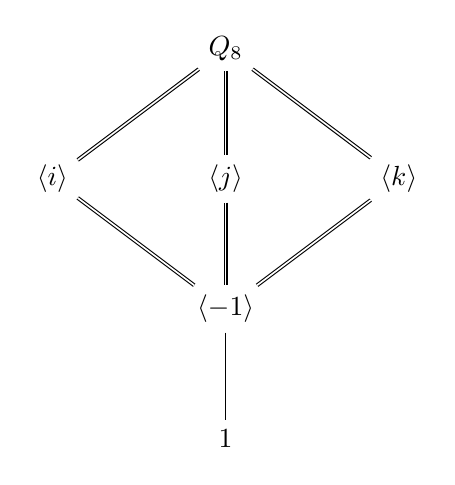
\begin{tikzpicture}[scale=1.1]
\node (top) at (0,3) {$Q_8$};
\node (i) at (-2,1.5) {$\langle i\rangle$};
\node (j) at (0,1.5) {$\langle j\rangle$};
\node (k) at (2,1.5) {$\langle k\rangle$};
\node (m) at (0,0) {$\langle -1\rangle$};
\node (bot) at (0,-1.5) {$1$};
\draw[double] (top)--(i);
\draw[double] (top)--(j);
\draw[double] (top)--(k);
\draw[double] (i)--(m);
\draw[double] (j)--(m);
\draw[double] (k)--(m);
\draw (m)--(bot);
\end{tikzpicture}
\end{center}

（2）同样的过程给出了 \(D_8/\langle r^2 \rangle\) 的格（双线）在 \(D_8\) 的格中的位置：

\begin{center}
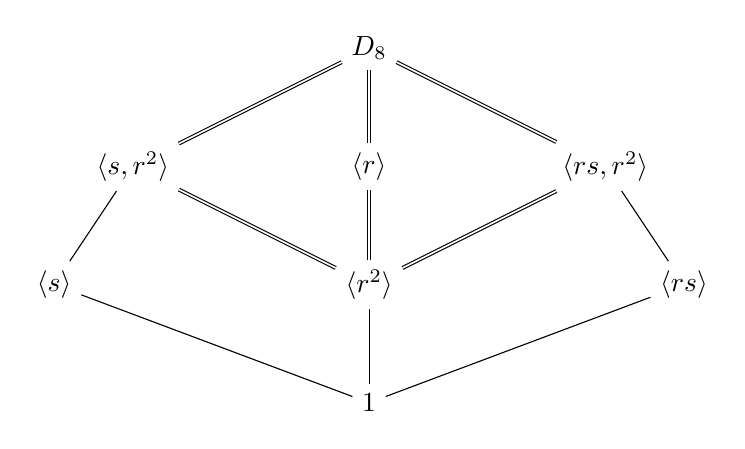
\begin{tikzpicture}[scale=1.0]
\node (top) at (0,4) {$D_8$};
\node (A) at (-3,2.5) {$\langle s, r^2\rangle$};
\node (B) at (0,2.5) {$\langle r\rangle$};
\node (C) at (3,2.5) {$\langle rs, r^2\rangle$};
\node (s) at (-4,1) {$\langle s\rangle$};
\node (m) at (0,1) {$\langle r^2\rangle$};
\node (rs) at (4,1) {$\langle rs\rangle$};
\node (bot) at (0,-0.5) {$1$};
\draw[double] (top)--(A);
\draw[double] (top)--(B);
\draw[double] (top)--(C);
\draw[double] (A)--(m);
\draw[double] (B)--(m);
\draw[double] (C)--(m);
\draw (A)--(s);
\draw (C)--(rs);
\draw (m)--(bot);
\draw (s)--(bot);
\draw (rs)--(bot);
\end{tikzpicture}
\end{center}

注意在上面第二个例子中，\(G\) 有些子群并不直接对应于商群 \(G/N\) 中的子群，即不含正规子群 \(N\) 的 \(G\) 的子群。这是因为子群 \(N\) 在 \(G/N\) 中被投影为一点，所以 \(G\) 的若干子群可以投影到商群中同一个子群。子群 \(H\) 在自然投影同态 \(G \to G/N\) 下的像与 \(G\) 的子群 \(HN\) 的像相同，而 \(G\) 的子群 \(HN\) 包含 \(N\). 反之，\(G/N\) 的子群 \(\bar{H}\) 的原像包含 \(N\)，并且是包含 \(N\) 的、在 \(G/N\) 中像为 \(\bar{H}\) 的唯一子群。正是包含 \(N\) 的 \(G\) 的子群在 \(G/N\) 的格中显式地出现。

上面两个 8 阶群的格强调了如下事实：一般不能仅由 \(G/N\) 和 \(N\) 的同构类型来确定一个群的同构类型，因为 \(Q_8/\langle -1 \rangle \cong D_8/\langle r^2 \rangle\) 且 \(\langle -1 \rangle \cong \langle r^2 \rangle\)，但 \(Q_8\) 与 \(D_8\) 不同构。我们将在下一节进一步讨论这个问题。

我们常常在子群格中用一个子群在另一个子群中的指数来标记，如下：

\begin{center}
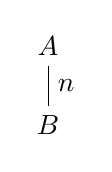
\begin{tikzpicture}[scale=1.0]
\node (A) at (0,1) {$A$};
\node (B) at (0,0) {$B$};
\draw (A)--node[right]{$n$}(B);
\end{tikzpicture}
\end{center}

其中整数 \(n\) 等于 \(|A : B|\). 例如，\(Q_8\) 和 \(D_8\) 的格中所有单线边都应标记为 2. 于是任意子群 \(A\) 的阶等于从单位元向上到 \(A\) 的任何一条路径上所有整数标记的乘积。此外，由定理 \ref{thm:3.20}(2)，这些指数在 \(G\) 对包含于 \(B\) 的正规子群取商时保持不变，即 \(G\) 的格中对应于商群格的那一部分，其指数对商群也是正确的。
\end{example}

最后我们给出一个关于在商群上定义同态的注记。在同构定理的证明过程中，我们遇到了这样的情况：商群 \(G/N\) 上的一个同态 \(\varphi\) 通过只借助代表元 \(g\) 给出它在陪集 \(gN\) 上的值来指定。在每种情形我们随后都必须证明 \(\varphi\) 良定义，即与 \(g\) 的选取无关。实际上，我们是在 \(G\) 本身上定义一个同态 \(\Phi\)，办法是指定 \(\Phi\) 在 \(g\) 处的值。此时，与 \(g\) 的选取无关等价于要求 \(\Phi\) 在 \(N\) 上是平凡的，因此
\[
\varphi \text{ 在 } G/N \text{ 上良定义} \iff N \subseteq \ker \Phi.
\]
这给出了在商群上定义同态的一个简单判别准则（即在 \(G\) 上定义一个同态，并验证 \(N\) 包含在它的核中）。在这种情形，我们说同态 \(\Phi\) \textbf{通过} \(N\) \textbf{分解}，而 \(\varphi\) 是 \(G/N\) 上的\textbf{诱导同态}。这可以用图 7 形象地表示，图中表明 \(\Phi = \varphi \circ \pi\)，即 \(G\) 中元素在 \(H\) 中的像不依赖于图中走哪条路径。若如此，则称该图\textbf{交换}。

\begin{center}
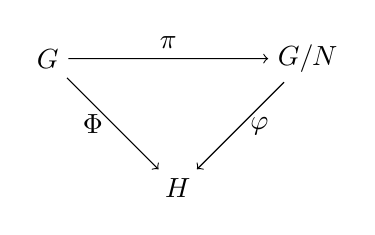
\begin{tikzpicture}[scale=1.1]
\node (G) at (0,2) {$G$};
\node (Q) at (3,2) {$G/N$};
\node (H) at (1.5,0.5) {$H$};
\draw[->] (G)--node[above]{$\pi$}(Q);
\draw[->] (G)--node[left]{$\Phi$}(H);
\draw[->] (Q)--node[right]{$\varphi$}(H);
\end{tikzpicture}

图 7
\end{center}

至此我们已经建立了全部背景材料，因此现在可以阅读 6.3 节关于自由群与表示的内容了。

\subsection*{习题}
设 \(G\) 是群。

\begin{enumerate}
\item 设 \(F\) 是 \(q\) 阶有限域，\(n \in \mathbb{Z}^+\). 证明 \(|GL_n(F) : SL_n(F)| = q - 1\).〔见第 2.1 节习题 35。〕

\item 证明格子同构定理的所有部分。

\item 证明：若 \(H\) 是 \(G\) 的指数为素数 \(p\) 的正规子群，则对任意 \(K \leq G\)，或者（i）\(K \leq H\)，或者（ii）\(G = HK\) 且 \(|K : K \cap H| = p\).

\item 设 \(C\) 是群 \(A\) 的正规子群，\(D\) 是群 \(B\) 的正规子群。证明 \(C \times D \trianglelefteq A \times B\) 且 \((A \times B)/(C \times D) \cong (A/C) \times (B/D)\).

\item 设 \(QD_{16} = \langle a, \tau \rangle\) 是第 2.5 节习题 11 中描述的拟二面体群。证明 \(\langle a^4 \rangle\) 在 \(QD_{16}\) 中正规，并用格子同构定理画出 \(QD_{16}/\langle a^4 \rangle\) 的子群格。哪个 8 阶群与本商群有相同的格？用 \(QD_{16}/\langle a^4 \rangle\) 的生成元与关系确定这个群的同构类型。

\item 设 \(M = \langle v, u \rangle\) 是第 2.5 节习题 14 中描述的 16 阶模群。证明 \(\langle v^4 \rangle\) 在 \(M\) 中正规，并用格子同构定理画出 \(M/\langle v^4 \rangle\) 的子群格。哪个 8 阶群与本商群有相同的格？用 \(M/\langle v^4 \rangle\) 的生成元与关系确定这个群的同构类型。

\item 设 \(M\) 和 \(N\) 是 \(G\) 的正规子群且 \(G = MN\). 证明 \(G/(M \cap N) \cong (G/M) \times (G/N)\).〔画出格。〕

\item 设 \(p\) 是素数，\(G\) 是 \(\mathbb{C}\) 中 1 的 \(p\) 次幂根构成的群（参见第 2.4 节习题 18）。证明映射 \(z \mapsto z^p\) 是满同态。由此推出 \(G\) 同构于它自身的一个真商群。

\item 设 \(p\) 是素数，\(G\) 是 \(p^\alpha m\) 阶群，其中 \(p\) 不整除 \(m\). 假设 \(P\) 是 \(G\) 的 \(p^\alpha\) 阶子群，\(N\) 是 \(G\) 的 \(p^\beta n\) 阶正规子群，其中 \(p\) 不整除 \(n\). 证明 \(|P \cap N| = p^\beta\) 且 \(|PN/N| = p^{\alpha - \beta}\).（\(G\) 的子群 \(P\) 称为 \(G\) 的\textbf{西罗 \(p\)-子群}。这个习题表明，\(G\) 的任意西罗 \(p\)-子群与正规子群 \(N\) 的交是 \(N\) 的西罗 \(p\)-子群。）

\item 按如下方式推广前一习题。有限群 \(G\) 的子群 \(H\) 称为 \(G\) 的\textbf{霍尔子群}，若它在 \(G\) 中的指数与它的阶互素：\((|G : H|, |H|) = 1\). 证明：若 \(H\) 是 \(G\) 的霍尔子群且 \(N \trianglelefteq G\)，则 \(H \cap N\) 是 \(N\) 的霍尔子群，且 \(HN/N\) 是 \(G/N\) 的霍尔子群。
\end{enumerate}

\section{合成列与赫尔德纲领}

上一节关于格的论述给我们留下了一个直观的图景：商群 \(G/N\) 是一个其结构（例如格）描述 \(N\) 之上 \(G\) 的结构的群。尽管这有些含糊，它至少给出了有限群论（甚至无限群论的某些分支）中最强有力的技巧之一——归纳法——背后的驱动力的某种概念。在许多情形下，归纳过程的应用遵循与下面柯西定理一个特殊情形的证明类似的模式。尽管柯西定理对任意群都成立（参见第 2 节的习题 9），下面这个证明是综合利用正规子群 \(N\) 和商群 \(G/N\) 的信息来确定关于 \(G\) 的信息的一个好例子，我们将在第 4 章用到这个特殊结果。

\begin{proposition}\label{pro:3.21}
若 \(G\) 是有限阿贝尔群，\(p\) 是整除 \(|G|\) 的素数，则 \(G\) 含 \(p\) 阶元素。
\end{proposition}

\begin{proof}
证明对 \(|G|\) 作归纳，即我们假设结论对阶严格小于 \(G\) 的阶的每个群成立，然后证明结论对 \(G\) 成立（这有时称为完全归纳法）。由于 \(|G| > 1\)，存在 \(x \in G\)，\(x \neq 1\). 若 \(|G| = p\)，则由拉格朗日定理 \(x\) 的阶为 \(p\)，结论得证。于是可设 \(|G| > p\).

假设 \(p\) 整除 \(|x|\)，写成 \(|x| = pn\). 由命题 2.5(3)，\(|x^n| = p\)，于是我们又有 \(p\) 阶元素。因此可设 \(p\) 不整除 \(|x|\).

令 \(N = \langle x \rangle\). 由于 \(G\) 阿贝尔，\(N \trianglelefteq G\). 由拉格朗日定理，\(|G/N| = \frac{|G|}{|N|}\)，且由于 \(N \neq 1\)，有 \(|G/N| < |G|\). 由于 \(p\) 不整除 \(|N|\)，必有 \(p \mid |G/N|\). 现在可以对较小的群 \(G/N\) 应用归纳假设，得出它含有一个 \(p\) 阶元素 \(\bar{y} = yN\). 由于 \(y \notin N\)（\(y \neq 1\)）但 \(y^p \in N\)（\(y^p = 1\)），必有 \(\langle y^p \rangle \neq \langle y \rangle\)，即 \(|y^p| < |y|\). 命题 2.5(2) 蕴含 \(p \mid |y|\). 现在我们就处于上一段所描述的情形，故那里的论证又产生一个 \(p\) 阶元素。归纳完成。
\end{proof}

这种方法背后的哲学是：如果对一个群 \(G\) 的某个正规子群 \(N\) 有足够多的信息，并且对 \(G/N\) 有足够多的信息，那么就可以把这些信息拼凑起来，迫使 \(G\) 本身具有某种所希望的性质。归纳法之所以起作用，是因为 \(N\) 和 \(G/N\) 的阶都比 \(G\) 小。一般说来，究竟需要多少数据是一个微妙的问题，因为正如我们已经看到的，仅由 \(N\) 和 \(G/N\) 的同构类型不能确定 \(G\) 的完整同构类型。

显然，这种方法的一个基本障碍是必须构造出 \(G\) 的一个非平凡真正规子群 \(N\)（即 \(N \neq 1, G\)）。在上面的论证中这很容易，因为 \(G\) 是阿贝尔群。没有非平凡真正规子群的群是这种方法的基本障碍。

\begin{definition}
群 \(G\)（有限或无限）称为\textbf{单群}，若 \(|G| > 1\) 且 \(G\) 的仅有的正规子群是 \(1\) 和 \(G\).
\end{definition}

由拉格朗日定理，若 \(|G|\) 是素数，则它仅有的子群（更不用说正规子群）是 \(1\) 和 \(G\)，故 \(G\) 是单群。事实上，每个阿贝尔单群都同构于某个素数 \(p\) 的 \(Z_p\)（参见习题 1）。存在非阿贝尔单群（有限阶和无限阶的都有），其中阶最小的为 60（我们将在下一节把这个群作为一无限族单群的成员引入）。

单群按定义不能被“分解”成像 \(N\) 和 \(G/N\) 这样的部分，因此它们扮演着类似于 \(\mathbb{Z}\) 的算术中素数的角色。这种类比得到了我们现在要描述的（有限群的）“唯一分解定理”的支持。

\begin{definition}
群 \(G\) 中的子群列
\[
1 = N_0 \trianglelefteq N_1 \trianglelefteq N_2 \trianglelefteq \cdots \trianglelefteq N_{k-1} \trianglelefteq N_k = G
\]
称为\textbf{合成列}，若 \(N_i \trianglelefteq N_{i+1}\) 且 \(N_{i+1}/N_i\) 是单群，\(0 \leq i \leq k-1\). 若上述序列是合成列，则商群 \(N_{i+1}/N_i\) 称为 \(G\) 的\textbf{合成因子}。
\end{definition}

请记住，这里并不假设每个 \(N_i \trianglelefteq G\)，只假设 \(N_i \trianglelefteq N_{i+1}\). 因此
\[
1 \trianglelefteq \langle s \rangle \trianglelefteq \langle s, r^2 \rangle \trianglelefteq D_8 \quad \text{和} \quad 1 \trianglelefteq \langle r^2 \rangle \trianglelefteq \langle r \rangle \trianglelefteq D_8
\]
是 \(D_8\) 的两个合成列，每个列中有 3 个合成因子，且每个都同构于（单群）\(Z_2\).

\begin{theorem}[若尔当-赫尔德]\label{thm:3.22}
设 \(G\) 是有限群且 \(G \neq 1\). 则

\begin{enumerate}[label=(\arabic*)]
\item \(G\) 有合成列；

\item 合成列中的合成因子是唯一的，即若
\[
1 = N_0 \trianglelefteq N_1 \trianglelefteq \cdots \trianglelefteq N_r = G \quad \text{和} \quad 1 = M_0 \trianglelefteq M_1 \trianglelefteq \cdots \trianglelefteq M_s = G
\]
是 \(G\) 的两个合成列，则 \(r = s\)，且存在 \(\{1, 2, \ldots, r\}\) 的一个置换 \(\sigma\) 使得 \(M_{\sigma(i)}/M_{\sigma(i)-1} \cong N_i/N_{i-1}\)，\(1 \leq i \leq r\).
\end{enumerate}
\end{theorem}

\begin{proof}
这相当直接。由于我们不会在正文中显式地用这个定理来证明其他结论，我们把证明作为本节末的一系列习题给出概要。
\end{proof}

因此每个有限群都有一个“分解”（即合成列），尽管列本身不必唯一（如 \(D_8\) 所示），但合成因子的个数及其同构类型是唯一确定的。此外，不同构的群可能有相同的（同构意义下）合成因子表（见习题 2）。这促使我们提出一个把所有有限群按同构分类的两部分纲领：

\textbf{赫尔德纲领}

（1）分类所有有限单群。

（2）找出把单群“拼在一起”形成其他群的所有方式。

这两个问题构成了群论许多发展的深层动机的一部分。这些问题的类似物也是贯穿整个数学的反复出现的主题。我们再补充一些关于这些问题进展现状的评论。

有限单群的分类（赫尔德纲领的第（1）部分）于 1980 年完成，距赫尔德纲领的提出约 100 年。100 多位数学家的工作、涵盖 5000 到 10000 页期刊论文（分布在约 300 到 500 篇单独论文中）证明了下面的结果：

\textbf{定理。} 存在一张由 18 个（无限）单群族和 26 个不属于这些族的单群（零星单群）组成的表，使得每个有限单群都同构于该表中的某个群。

一个单群族的例子是 \(\{Z_p \mid p \text{ 是素数}\}\). 有限单群表中的第二个无限族是：
\[
\{SL_n(\mathbb{F})/Z(SL_n(\mathbb{F})) \mid n \in \mathbb{Z}^+,\ n \geq 2,\ \mathbb{F} \text{ 是有限域}\}.
\]
除 \(SL_2(\mathbb{F}_2)\) 和 \(SL_2(\mathbb{F}_3)\) 外（其中 \(\mathbb{F}_2\) 是含 2 个元素的有限域，\(\mathbb{F}_3\) 是含 3 个元素的有限域），这些群都是单群。这是一个二参数族（\(n\) 和 \(\mathbb{F}\) 是独立的参数）。我们不证明这些群是单群（尽管这在技术上并未超出本书的范围），而是请读者参考 Finite Group Theory（M. Aschbacher 著，Cambridge University Press, 1986）一书，其中有证明以及对单群问题的详尽讨论。第三个有限单群族（交错群）将在下一节讨论；我们将在下一章证明这些群是单群。

为了对有限单群分类的复杂性有所了解，读者不妨浏览一下整个分类的一块基石（Feit--Thompson 定理）的证明：

\textbf{定理（Feit--Thompson）。} 若 \(G\) 是奇数阶单群，则 \(G \cong Z_p\)，其中 \(p\) 为某个素数。

这个证明用了 255 页艰深的数学\footnote{Solvability of groups of odd order, Pacific Journal of Mathematics, 13(1963), pp. 775--1029.}。

赫尔德纲领的第（2）部分有时称为\textbf{扩张问题}，其表述相当含糊。对“把两个群拼在一起”更精确的描述是：给定群 \(A\) 和 \(B\)，描述如何得到所有含正规子群 \(N\) 的群 \(G\)，使得 \(N \cong B\) 且 \(G/N \cong A\). 例如，若 \(A = B = Z_2\)，则 \(G\) 恰好有两种可能，即 \(Z_4\) 和 \(V_4\)（见第 2.5 节习题 10），而赫尔德纲领试图描述如何在不预先知道 4 阶群存在的情况下，由两个 \(Z_2\) 构造出这两个 4 阶群。赫尔德纲领的这一部分极其困难，即使所涉及的子群阶很小。例如，群 \(G\) 的所有合成因子都是 2 阶的，当且仅当 \(|G| = 2^n\)（一个方向容易，我们将在第 6 章证明两个方向）。然而已知，\(2^n\) 阶不同构的群的个数随 \(2^n\) 增长（指数式增长），所以把 2 幂阶群拼在一起的方式数不受限制。尽管如此，在这个微妙的领域中有大量有趣而强有力的技巧，可用来揭示许多类群的结构。我们将只讨论从较小群构造较大群（在上述意义下）的少数几种方式，但即便从对群扩张这个领域的这一有限涉猎中，我们也将在构造大量新群例子并证明一些分类定理。

在多项式方程理论中起突出作用的一类群是可解群：

\begin{definition}
群 \(G\) 称为\textbf{可解}的，若存在子群链
\[
1 = G_0 \trianglelefteq G_1 \trianglelefteq G_2 \trianglelefteq \cdots \trianglelefteq G_s = G
\]
使得 \(G_{i+1}/G_i\) 是阿贝尔群，\(i = 0, 1, \ldots, s-1\).
\end{definition}

这个术语来自伽罗瓦理论中这些群与可由根式求解的多项式之间的对应（这本质上意味着存在根的代数公式）。习题 8 表明，有限可解群恰好就是那些所有合成因子都是素数阶的群。

有限可解群的一个引人注目的性质是下面这个由 Philip Hall 给出的西罗定理的推广（参见定理 6.11 和定理 19.8）。

\textbf{定理。} 有限群 \(G\) 可解，当且仅当对 \(|G|\) 的每个满足 \(\left(n, \frac{|G|}{n}\right) = 1\) 的因子 \(n\)，\(G\) 都有 \(n\) 阶子群。

作为群的性性质如何由正规子群 \(N\) 和商群 \(G/N\) 的信息综合推得的另一个例子，我们证明：若 \(N\) 和 \(G/N\) 可解，则 \(G\) 可解。

为此，设 \(\bar{G} = G/N\)，设 \(1 = N_0 \trianglelefteq N_1 \trianglelefteq \cdots \trianglelefteq N_n = N\) 是 \(N\) 的子群链，使得 \(N_{i+1}/N_i\) 是阿贝尔群（\(0 \le i < n\)），并设 \(1 = \bar{G}_0 \trianglelefteq \bar{G}_1 \trianglelefteq \cdots \trianglelefteq \bar{G}_m = \bar{G}\) 是 \(\bar{G}\) 的子群链，使得 \(\bar{G}_{i+1}/\bar{G}_i\) 是阿贝尔群（\(0 \le i < m\)）。由格子同构定理，存在 \(G\) 的子群 \(G_i\) 使得 \(N \leq G_i\)、\(G_i/N = \bar{G}_i\) 且 \(G_i \trianglelefteq G_{i+1}\)，\(0 \le i < m\). 由第三同构定理
\[
G_{i+1}/G_i \cong (G_{i+1}/N)/(G_i/N) = \bar{G}_{i+1}/\bar{G}_i
\]
是阿贝尔群。因此
\[
1 = N_0 \trianglelefteq N_1 \trianglelefteq \cdots \trianglelefteq N_n = N = G_0 \trianglelefteq G_1 \trianglelefteq \cdots \trianglelefteq G_m = G
\]
是 \(G\) 的一个子群链，其所有相继商群都是阿贝尔群。这证明 \(G\) 可解。

说有限群论只关心赫尔德纲领是不准确的。准确的说法是，赫尔德纲领提出了大量问题并推动了许多代数技巧。例如，在扩张问题中，给定群 \(A\) 和 \(B\)，希望找到 \(G\) 和 \(N \trianglelefteq G\) 使得 \(N \cong B\)、\(G/N \cong A\)，我们将看到（在一定条件下）这引导我们得到群 \(A\) 在集合 \(B\) 上的一个作用。这类作用是下一章的核心（并将给出关于单群和非单群的信息），而且这一概念在数学中是一个强有力的概念，并不限于群论。本章最后一节引入另一族群，它虽然符合我们对单群的兴趣，但将在全书中具有独立的重要性，特别是在我们后面研究行列式和多项式方程的可解性时。

\subsection*{习题}
设 \(G\) 是群。

\begin{enumerate}
\item 证明：若 \(G\) 是阿贝尔单群，则 \(G \cong Z_p\)，其中 \(p\) 为某个素数（不要假设 \(G\) 是有限群）。

\item 列出 \(Q_8\) 的所有 3 个合成列和 \(D_8\) 的所有 7 个合成列。写出每种情形的合成因子。

\item 求 16 阶拟二面体群的一个合成列（参见第 2.5 节习题 11）。由此推出 \(QD_{16}\) 可解。

\item 用柯西定理和归纳法证明：有限阿贝尔群对其阶的每个正因子 \(n\) 都有 \(n\) 阶子群。

\item 证明可解群的子群和商群可解。

\item 对 \(|G|\) 作归纳，证明若尔当-赫尔德定理的第（1）部分。

\item 若 \(G\) 是有限群且 \(H \trianglelefteq G\)，证明存在 \(G\) 的一个合成列，其中某一项是 \(H\).

\item 设 \(G\) 是有限群。证明下列命题等价：

（i）\(G\) 可解；

（ii）\(G\) 有子群链 \(1 = H_0 \trianglelefteq H_1 \trianglelefteq H_2 \trianglelefteq \cdots \trianglelefteq H_s = G\)，使得 \(H_{i+1}/H_i\) 是循环群，\(0 \leq i \leq s-1\)；

（iii）\(G\) 的所有合成因子都是素数阶的；

（iv）\(G\) 有子群链 \(1 = N_0 \trianglelefteq N_1 \trianglelefteq \cdots \trianglelefteq N_t = G\)，使得每个 \(N_i\) 是 \(G\) 的正规子群且 \(N_{i+1}/N_i\) 是阿贝尔群，\(0 \leq i \leq t-1\).

〔对（iv），先证明 \(G\) 的极小非平凡正规子群 \(M\) 必阿贝尔，然后用归纳法。为看出 \(M\) 阿贝尔，取 \(N \trianglelefteq M\) 具有素数指数（由（iii）），并证明对所有 \(y \in M\) 有 \(x^{-1}y^{-1}xy \in N\)（参见第 1 章习题 40）。把同样的论证用于 \(gNg^{-1}\)，证明 \(x^{-1}y^{-1}xy\) 属于 \(N\) 的所有 \(G\)-共轭的交，并利用 \(M\) 的极小性推出 \(x^{-1}y^{-1}xy = 1\).〕

\item 证明若尔当-赫尔德定理第（2）部分的如下特殊情形：假设有限群 \(G\) 有两个合成列
\[
1 = N_0 \trianglelefteq N_1 \trianglelefteq \cdots \trianglelefteq N_r = G \quad \text{和} \quad 1 = M_0 \trianglelefteq M_1 \trianglelefteq M_2 = G.
\]
证明 \(r = 2\) 且合成因子表相同。〔使用第二同构定理。〕

\item 对 \(\min\{r, s\}\) 作归纳，证明若尔当-赫尔德定理的第（2）部分。〔对 \(H = N_{r-1} \cap M_{s-1}\) 应用归纳假设，并利用前面几个习题。〕

\item 证明：若 \(H\) 是可解群 \(G\) 的非平凡正规子群，则存在 \(H\) 的非平凡子群 \(A\) 使得 \(A \trianglelefteq G\) 且 \(A\) 阿贝尔。

\item 证明（不使用 Feit--Thompson 定理）下列命题等价：

（i）每个奇数阶群都可解；

（ii）奇数阶单群只有素数阶的那些。
\end{enumerate}

\section{对换与交错群}

\subsection*{对换与 \(S_n\) 的生成}

如我们在第 1.3 节所见（并将在下一章证明），\(S_n\) 的每个元素都可以本质上唯一地写成不交循环的乘积。相反，\(S_n\) 的每个元素都可以用许多不同的方式写成（不必不交的）循环的乘积。例如，即使在 \(S_3\) 中，元素 \(\sigma = (1\,2\,3)\) 也可以写成
\[
\sigma = (1\,2\,3) = (1\,3)(1\,2) = (1\,2)(1\,3)(1\,2)(1\,3) = (1\,2)(2\,3),
\]
事实上，\(\sigma\) 有无穷多种不同的写法。不要求循环不交，完全破坏了置换表示为循环乘积的唯一性。然而，我们可以通过把置换（非唯一地）写成 2-循环的乘积而得到某种“奇偶性检验”。

\begin{definition}
2-循环称为\textbf{对换}。
\end{definition}

直观上，\(\{1, 2, \ldots, n\}\) 的每个置换都可以通过一系列对换、即简单交换若干对元素来实现（不妨拿一副小牌试试！）。我们来说明如何做到这一点。首先注意，对任何 \(m\)-循环，
\[
(a_1\, a_2\, \ldots\, a_m) = (a_1\, a_m)(a_1\, a_{m-1})(a_1\, a_{m-2}) \cdots (a_1\, a_2).
\]
现在 \(S_n\) 中任何置换都可以写成循环的乘积（例如它的循环分解）。依次用上面的方法把每个循环写成对换的乘积，我们看到：\(S_n\) 的每个元素都可以写成对换的乘积；或者等价地，
\[
S_n = \langle T \rangle, \quad \text{其中 } T = \{(i\, j) \mid 1 \leq i < j \leq n\}.
\]
例如，第 1.3 节中的置换 \(\sigma\) 可以写成
\[
\sigma = (1\, 12\, 8\, 10\, 4)(2\, 13)(5\, 11\, 7)(6\, 9) = (1\, 4)(1\, 10)(1\, 8)(1\, 12)(2\, 13)(5\, 7)(5\, 11)(6\, 9).
\]

\subsection*{交错群}

我们再次强调，对任意 \(\sigma \in S_n\)，把 \(\sigma\) 写成对换乘积的方式可能有很多种。对固定的 \(\sigma\)，我们现在证明：任何等于 \(\sigma\) 的对换乘积都具有相同的奇偶性（即项数为奇数或偶数）。

设 \(x_1, \ldots, x_n\) 是独立变量，令 \(\Delta\) 为多项式
\[
\Delta = \prod_{1 \leq i < j \leq n} (x_i - x_j),
\]
即所有 \(i < j\) 的项 \(x_i - x_j\) 的乘积。例如，当 \(n = 4\) 时，
\[
\Delta = (x_1 - x_2)(x_1 - x_3)(x_1 - x_4)(x_2 - x_3)(x_2 - x_4)(x_3 - x_4).
\]
对每个 \(\sigma \in S_n\)，让 \(\sigma\) 以它与置换下标相同的方式置换变量来作用于 \(\Delta\)：
\[
\sigma(\Delta) = \prod_{1 \leq i < j \leq n} (x_{\sigma(i)} - x_{\sigma(j)}).
\]
例如，若 \(n = 4\) 且 \(\sigma = (1\,2\,3\,4)\)，则
\[
\sigma(\Delta) = (x_2 - x_3)(x_2 - x_4)(x_2 - x_1)(x_3 - x_4)(x_3 - x_1)(x_4 - x_1)
\]
（我们按与上面相同的顺序写出各个因子，并对每个因子作用 \(\sigma\) 得到 \(\sigma(\Delta)\)）。一般地注意，对所有 \(i < j\)，\(\Delta\) 含有一个因子 \(x_i - x_j\)；由于 \(\sigma\) 是下标的一个双射，\(\sigma(\Delta)\) 对所有 \(i < j\) 必含有 \(x_i - x_j\) 或 \(x_j - x_i\) 之一，但不会同时含有（当然也不会含有 \(x_i - x_i\) 这样的项）。若 \(\sigma(\Delta)\) 含有形如 \(x_j - x_i\)（\(j > i\)）的因子，就把这一项写成 \(-(x_i - x_j)\). 把所有符号变化收集起来，我们看到 \(\Delta\) 与 \(\sigma(\Delta)\) 的因子相同，至多相差若干个 \(-1\) 的乘积，即
\[
\sigma(\Delta) = \pm\Delta, \quad \text{对所有 } \sigma \in S_n.
\]
对每个 \(\sigma \in S_n\)，令
\[
\varepsilon(\sigma) = \begin{cases} +1, & \text{若 } \sigma(\Delta) = \Delta, \\ -1, & \text{若 } \sigma(\Delta) = -\Delta. \end{cases}
\]
在上面 \(n = 4\)、\(\sigma = (1\,2\,3\,4)\) 的例子中，\(\sigma(\Delta)\) 中恰好有 3 个形如 \(x_j - x_i\)（\(j > i\)）的因子，每个贡献一个因子 \(-1\). 因此
\[
(1\,2\,3\,4)(\Delta) = (-1)^3 \Delta = -\Delta,
\]
所以
\[
\varepsilon((1\,2\,3\,4)) = -1.
\]

\begin{definition}
（1）\(\varepsilon(\sigma)\) 称为 \(\sigma\) 的\textbf{符号}。

（2）若 \(\varepsilon(\sigma) = 1\) 则称 \(\sigma\) 为\textbf{偶置换}，若 \(\varepsilon(\sigma) = -1\) 则称 \(\sigma\) 为\textbf{奇置换}。
\end{definition}

下一个结果表明置换的符号定义了一个同态。

\begin{proposition}\label{pro:3.23}
映射 \(\varepsilon : S_n \to \{\pm 1\}\) 是同态（这里 \(\{\pm 1\}\) 是 2 阶循环群的乘法版本）。
\end{proposition}

\begin{proof}
按定义，
\[
(\tau\sigma)(\Delta) = \prod_{1 \leq i < j \leq n} (x_{\tau\sigma(i)} - x_{\tau\sigma(j)}).
\]
假设 \(\sigma(\Delta)\) 中恰有 \(k\) 个形如 \(x_j - x_i\)（\(j > i\)）的因子，即 \(\varepsilon(\sigma) = (-1)^k\). 在计算 \((\tau\sigma)(\Delta)\) 时，先对下标作用 \(\sigma\)，我们看到 \((\tau\sigma)(\Delta)\) 中恰有 \(k\) 个形如 \(x_{\tau(j)} - x_{\tau(i)}\)（\(j > i\)）的因子。交换这 \(k\) 个因子中各项的次序引入符号变化 \((-1)^k = \varepsilon(\sigma)\)，此时 \((\tau\sigma)(\Delta)\) 的所有因子都形如 \(x_{\tau(p)} - x_{\tau(q)}\)（\(p < q\)）。因此
\[
(\tau\sigma)(\Delta) = \varepsilon(\sigma) \prod_{1 \leq p < q \leq n} (x_{\tau(p)} - x_{\tau(q)}).
\]
由 \(\varepsilon\) 的定义，
\[
\prod_{1 \leq p < q \leq n} (x_{\tau(p)} - x_{\tau(q)}) = \varepsilon(\tau)\Delta,
\]
故 \((\tau\sigma)(\Delta) = \varepsilon(\sigma)\varepsilon(\tau)\Delta\). 因此 \(\varepsilon(\tau\sigma) = \varepsilon(\sigma)\varepsilon(\tau) = \varepsilon(\tau)\varepsilon(\sigma)\)，如所断言。
\end{proof}

为看清这个证明的实际运作，设 \(n = 4\)、\(\sigma = (1\,2\,3\,4)\)、\(\tau = (4\,2\,3)\)，故 \(\tau\sigma = (1\,3\,2\,4)\). 按定义（使用本例中显式的 \(\Delta\)），
\[
(\tau\sigma)(\Delta) = (1\,3\,2\,4)(\Delta) = (x_3 - x_4)(x_3 - x_2)(x_3 - x_1)(x_4 - x_2)(x_4 - x_1)(x_2 - x_1) = (-1)^5 \Delta,
\]
其中除第一个因子外所有因子都被翻转以恢复 \(\Delta\). 这表明 \(\varepsilon(\tau\sigma) = -1\). 另一方面，由于我们已经算过 \(\sigma(\Delta)\)，
\[
\begin{aligned}
(\tau\sigma)(\Delta) = \tau(\sigma(\Delta)) &= (x_{\tau(2)} - x_{\tau(3)})(x_{\tau(2)} - x_{\tau(4)})(x_{\tau(2)} - x_{\tau(1)})(x_{\tau(3)} - x_{\tau(4)}) \\
&\quad \times (x_{\tau(3)} - x_{\tau(1)})(x_{\tau(4)} - x_{\tau(1)}) \\
&= (-1)^3 \prod_{1 \leq p < q \leq 4} (x_{\tau(p)} - x_{\tau(q)}) = (-1)^3 \tau(\Delta),
\end{aligned}
\]
其中第三个、第五个和第六个因子需要交换各项的次序，才能把所有因子写成 \(x_{\tau(p)} - x_{\tau(q)}\)（\(p < q\)）的形式。我们已经算出 \(\varepsilon(\sigma) = (-1)^3 = -1\)，用同样的方法容易看出 \(\varepsilon(\tau) = (-1)^2 = 1\)，所以 \(\varepsilon(\tau\sigma) = -1 = \varepsilon(\tau)\varepsilon(\sigma)\).

下一步是对任意对换 \((i\, j)\) 计算 \(\varepsilon((i\, j))\). 与其对任意 \(i, j\) 直接计算，我们先对 \(i = 1, j = 2\) 计算，再把一般情形归约到它。显然，把 \((1\,2)\) 作用于 \(\Delta\)（无论 \(n\) 是多少）恰好翻转一个因子，即 \(x_1 - x_2\)；因此 \(\varepsilon((1\,2)) = -1\). 现在对任意对换 \((i\, j)\)，设 \(\lambda\) 是交换 1 与 \(i\)、交换 2 与 \(j\)、并固定其余所有数的置换（若 \(i = 1\) 或 \(j = 2\)，则 \(\lambda\) 分别固定 \(i\) 或 \(j\)）。那么容易看出 \((i\, j) = \lambda(1\,2)\lambda\)（计算右端对任意 \(k \in \{1, 2, \ldots, n\}\) 的作用）。由于 \(\varepsilon\) 是同态，我们得到
\[
\varepsilon((i\, j)) = \varepsilon(\lambda(1\,2)\lambda) = \varepsilon(\lambda)\varepsilon((1\,2))\varepsilon(\lambda) = (-1)\varepsilon(\lambda)^2 = -1.
\]
这证明了

\begin{proposition}\label{pro:3.24}
对换都是奇置换，且 \(\varepsilon\) 是满同态。
\end{proposition}

\begin{definition}
\(n\) 次\textbf{交错群}，记作 \(A_n\)，是同态 \(\varepsilon\) 的核（即偶置换的集合）。
\end{definition}

注意由第一同构定理，\(S_n/A_n \cong \varepsilon(S_n) = \{\pm 1\}\)，所以 \(A_n\) 的阶容易确定：\(|A_n| = \frac{1}{2}|S_n| = \frac{1}{2}(n!)\). 此外，\(S_n - A_n\) 是 \(A_n\) 的非单位陪集，它是所有奇置换的集合。置换的符号服从通常的 \(\mathbb{Z}/2\mathbb{Z}\) 法则：
\[
(\text{偶})(\text{偶}) = (\text{奇})(\text{奇}) = \text{偶}, \qquad (\text{偶})(\text{奇}) = (\text{奇})(\text{偶}) = \text{奇}.
\]
此外，由于 \(\varepsilon\) 是同态且每个 \(\sigma \in S_n\) 是对换的乘积，设 \(\sigma = \tau_1\tau_2\cdots\tau_k\)，则 \(\varepsilon(\sigma) = \varepsilon(\tau_1)\cdots\varepsilon(\tau_k)\)；由于 \(\varepsilon(\tau_i) = -1\)（\(i = 1, 2, \ldots, k\)），故 \(\varepsilon(\sigma) = (-1)^k\). 因此 \(k \bmod 2\) 这一等价类、即乘积中对换个数的奇偶性，无论我们怎样把 \(\sigma\) 写成对换的乘积都是相同的：
\[
\varepsilon(\sigma) = \begin{cases} +1, & \text{若 } \sigma \text{ 是偶数个对换的乘积}, \\ -1, & \text{若 } \sigma \text{ 是奇数个对换的乘积}. \end{cases}
\]
最后我们给出一个由 \(\sigma\) 的循环分解快速计算 \(\varepsilon(\sigma)\) 的方法。回忆一个 \(m\)-循环可以写成 \(m - 1\) 个对换的乘积。因此 \(m\)-循环是奇置换当且仅当 \(m\) 是偶数。

对任意置换 \(\sigma\)，设 \(\sigma_1\sigma_2\cdots\sigma_k\) 是它的循环分解。则 \(\varepsilon(\sigma)\) 由 \(\varepsilon(\sigma_1)\cdots\varepsilon(\sigma_k)\) 给出，而 \(\varepsilon(\sigma_i) = -1\) 当且仅当 \(\sigma_i\) 的长度为偶数。由此推出，为使 \(\varepsilon(\sigma) = -1\)，诸 \(\varepsilon(\sigma_i)\) 的乘积中必须含有奇数个因子 \((-1)\). 我们把它总结为下面的命题：

\begin{proposition}\label{pro:3.25}
置换 \(\sigma\) 是奇置换，当且仅当它的循环分解中偶长度循环的个数为奇数。
\end{proposition}

例如，\(\sigma = (1\,2\,3\,4\,5\,6)(7\,8\,9)(10\,11)(12\,13\,14\,15)(16\,17\,18)\) 有 3 个偶长度循环，故 \(\varepsilon(\sigma) = -1\). 另一方面，\(\tau = (1\,12\,8\,10\,4)(2\,13)(5\,11\,7)(6\,9)\) 恰有 2 个偶长度循环，故 \(\varepsilon(\tau) = 1\).

注意不要把置换 \(\sigma\) 的“奇”“偶”与 \(\sigma\) 的阶的奇偶性相混淆。事实上，若 \(\sigma\) 的阶为奇数，则 \(\sigma\) 的循环分解中所有循环都有奇数长度，所以 \(\sigma\) 有偶数个（此时为 0 个）偶长度循环，从而是偶置换。若 \(|\sigma|\) 是偶数，则 \(\sigma\) 可以是偶置换也可以是奇置换；例如 \((1\,2)\) 是奇置换，\((1\,2)(3\,4)\) 是偶置换，但二者的阶都是 2.

如上一节提到的，交错群 \(A_n\) 将在多项式可解性的研究中起重要作用。下一章我们将证明：

\begin{center}
\(A_n\) 对所有 \(n \geq 5\) 都是非阿贝尔单群。
\end{center}

对小 \(n\) 值，\(A_n\) 已经为我们所熟悉：\(A_1\) 和 \(A_2\) 都是平凡群，\(|A_3| = 3\)（故 \(A_3 = \langle (1\,2\,3) \rangle \cong Z_3\)）。群 \(A_4\) 的阶为 12. 习题 7 表明 \(A_4\) 同构于正四面体的对称群。\(A_4\) 的子群格出现在图 8 中（习题 8 断言这是它完整的子群格）。这个格比较好的方面之一是，它（不像“几乎所有群”的格那样）是一个平面图（除顶点外没有交叉的线；可比较 \(D_{16}\) 的非平面格）。

\begin{center}
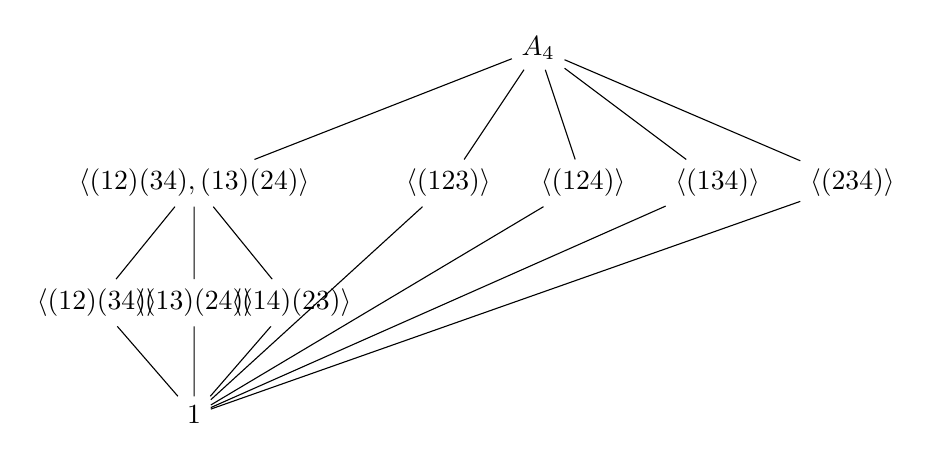
\begin{tikzpicture}[scale=0.95]
\node (top) at (0,4) {$A_4$};
\node (V) at (-4.6,2.2) {$\langle(12)(34),(13)(24)\rangle$};
\node (c1) at (-1.2,2.2) {$\langle(123)\rangle$};
\node (c2) at (0.6,2.2) {$\langle(124)\rangle$};
\node (c3) at (2.4,2.2) {$\langle(134)\rangle$};
\node (c4) at (4.2,2.2) {$\langle(234)\rangle$};
\node (d1) at (-5.9,0.6) {$\langle(12)(34)\rangle$};
\node (d2) at (-4.6,0.6) {$\langle(13)(24)\rangle$};
\node (d3) at (-3.3,0.6) {$\langle(14)(23)\rangle$};
\node (bot) at (-4.6,-0.9) {$1$};
\draw (top)--(V);
\draw (top)--(c1);
\draw (top)--(c2);
\draw (top)--(c3);
\draw (top)--(c4);
\draw (V)--(d1);
\draw (V)--(d2);
\draw (V)--(d3);
\draw (d1)--(bot);
\draw (d2)--(bot);
\draw (d3)--(bot);
\draw (c1)--(bot);
\draw (c2)--(bot);
\draw (c3)--(bot);
\draw (c4)--(bot);
\end{tikzpicture}

图 8
\end{center}

\subsection*{习题}

\begin{enumerate}
\item 在第 1.3 节的习题 1 和 2 中，你被要求求一些置换的循环分解。把这些置换中的每一个写成对换的乘积。判断其中哪些是偶置换，哪些是奇置换。

\item 证明对每个置换 \(\sigma\)，\(\sigma^2\) 都是偶置换。

\item 证明 \(S_n\) 由 \(\{(i\ i+1) \mid 1 \leq i \leq n-1\}\) 生成。〔考虑共轭，即 \((2\,3)(1\,2)(2\,3)^{-1}\).〕

\item 证明对所有 \(n \geq 2\)，\(S_n = \langle (1\,2), (1\,2\,\ldots\,n) \rangle\).

\item 证明：若 \(p\) 是素数，则 \(S_p = \langle \sigma, \tau \rangle\)，其中 \(\sigma\) 是任意对换，\(\tau\) 是任意 \(p\)-循环。

\item 证明 \(\langle (1\,3), (1\,2\,3\,4) \rangle\) 是 \(S_4\) 的真子群。这个子群的同构类型是什么？

\item 证明正四面体的刚体运动群同构于 \(A_4\).〔回忆第 1.7 节习题 20。〕

\item 证明正文中给出的 \(A_4\) 的子群格是正确的。〔由前一习题和拉格朗日定理之后的评注，\(A_4\) 没有 6 阶子群。〕

\item 证明 \(A_4\) 中（唯一的）4 阶子群正规，且同构于 \(V_4\).

\item 求 \(A_4\) 的一个合成列。由此推出 \(A_4\) 可解。

\item 证明 \(S_4\) 没有同构于 \(Q_8\) 的子群。

\item 证明对每个 \(n \geq 3\)，\(A_n\) 含有一个同构于 \(S_{n-2}\) 的子群。

\item 证明 \(A_n\) 中每个 2 阶元素都是 \(S_n\) 中某个 4 阶元素的平方。〔\(A_n\) 中的 2 阶元素是 \(2k\) 个彼此交换的对换的乘积。〕

\item 证明 \(A_4\) 中由任意一个 2 阶元素和任意一个 3 阶元素生成的子群是整个 \(A_4\).

\item 证明：若 \(x\) 和 \(y\) 是 \(S_4\) 中不同的 3-循环且 \(x \neq y^{-1}\)，则由 \(x\) 和 \(y\) 生成的 \(S_4\) 的子群是 \(A_4\).

\item 设 \(x\) 和 \(y\) 是 \(S_5\) 中不同的 3-循环且 \(x \neq y^{-1}\).

（a）证明：若 \(x\) 和 \(y\) 固定 \(\{1, \ldots, 5\}\) 的一个公共元素，则 \(\langle x, y \rangle \cong A_4\).

（b）证明：若 \(x\) 和 \(y\) 不固定 \(\{1, \ldots, 5\}\) 的公共元素，则 \(\langle x, y \rangle = A_5\).

\item 若 \(x\) 和 \(y\) 是 \(S_n\) 中的 3-循环，证明 \(\langle x, y \rangle\) 同构于 \(Z_3\)、\(A_4\)、\(A_5\) 或 \(Z_3 \times Z_3\).
\end{enumerate}
